

\part{Introducción al diseño de filtros activos}
\section{Introducción teórica del \textit{Gyrator}}
El concepto de \textit{Gyrator} fue introducido en 1948 por Bernard D.H.Tellegen como el hipotético quinto elemento linear luego del capacitor, inductor, resistencia y
el transformador ideal. Es un elemento electrónico de dos puertas no reciproco cuyo símbolo se puede ver en la Figura \ref{ej2_gyrator_symbol}.

\begin{figure}[h!]                                                       
    \centering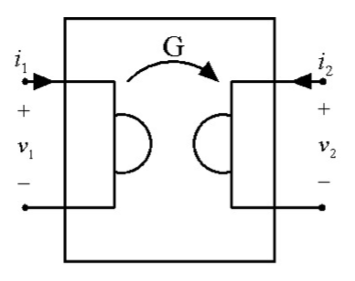
\includegraphics[width=0.4\textwidth, height=4cm]{../Ex2/Resources/ej2_gyrator_symbol.png}
    \caption{Símbolo del \textit{Gyrator}}
    \label{ej2_gyrator_symbol}
    \end{figure}

El coeficiente $G$ tiene dimensiones de $\frac{1}{\Omega}$ y por ello se le da el nombre de \textit{Gyrator conductance}. Luego, su inversa $\frac{1}{G} = R$ se define como \textit{Gyrator resistance}. Esta resistencia tiene una direccion asociada que 
se indica por una flecha, como se puede apreciar en la Figura \ref{ej2_gyrator_symbol}. Invertir el sentido de la flecha es negar la resistencia del \textit{Gyrator} o que es lo mismo que invertir
la polaridad del puerto. A continuación se definen las ecuaciones del \textit{Gyrator} , que se depreden de la figura anteriormente mencionada:

\begin{equation} I_{1} = G V_2 \label{ej2_ecua_gyrator_1}\end{equation}
\begin{equation} I_{2} =  -G V_1 \label{ej2_ecua_gyrator_2}\end{equation}


Gracias (\ref{ej2_ecua_gyrator_1}) y (\ref{ej2_ecua_gyrator_2}) se pueden enumerar las siguientes propiedades de un \textit{Gyrator} ideal:    

\begin{enumerate}
	\item Potencia instantánea nula \\
        \begin{displaymath} P = V_1 I_1 + V_2 I_2 \end{displaymath}
        \begin{displaymath} P = (-G I_2)I_1 + (G I_1) I_2 \end{displaymath}
        \begin{displaymath} P = 0 \end{displaymath}
    
	\item Parámetros de impedancia $Z$ y parámetros de admitancia $Y$ \\
        %poner las matrices Z y Y. Es necesario ?????
	\item Inversión de impedancia de elementos lineales\\
        Si se conecta una impedancia $Z_2$ en las terminales de salida del \textit{Gyrator} y $Z_1$ es la impedancia en las terminales de entrada, se deduce lo siguiente:
        \begin{displaymath} Z_2 = \frac{V_2}{-I_2} \end{displaymath}
        \begin{displaymath} \frac{V_2}{-I_2} = \frac{\frac{-I_1}{G}}{ -G V_1} \end{displaymath}
        \begin{displaymath} \frac{V_2}{I_2} = \frac{I_1}{G^2 V_1} \end{displaymath}
        \begin{displaymath} Z_2 = \frac{1}{Z_1 G^2} \end{displaymath}
        \begin{displaymath} Z_1 = \frac{1}{Z_2 G^2} \end{displaymath}

        Esto implica que si se conecta, por ejemplo, una resistencia lineal $R_L$ en las terminales de salida del \textit{Gyrator}, la entrada se comporta como
        una resistencia lineal de impedancia $ \frac{1}{R_L G^2} $. Luego, se puede lograr que una capacidad se comporte como una inductancia. Esta propiedad es sumamente interesante
        ya que se puede utilizar al \textit{Gyrator} para realizar filtros sin inductores. Antes del desarrollo del transistor, los inductores eran grandes y costosos por lo que su uso traían varios problemas. Gracias al \textit{Gyrator}
        se puede sustituir al inductor y sobrepasar este tipo de problemas. Esta propiedad es la que mas se utiliza a lo largo de toda esta sección. La Figura \ref{ej2_gyrator_prop2} muestra esta propiedad.
        Nótese que, un capacitor de valor $C$ a la salida de un \textit{Gyrator} ideal hace que a la entrada halla una inductancia igual a:

        \begin{equation} L =  \frac{C}{G^2} \label{ej2_ecua_gyrator_inversion_impedancia}\end{equation}

        \begin{figure}[h!]                                                       
            \centering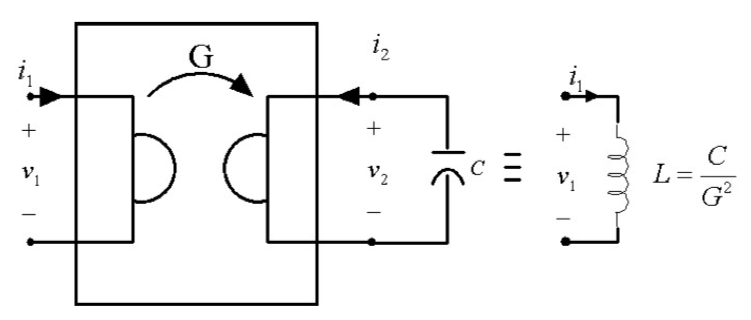
\includegraphics[width=0.7\textwidth, height=4cm]{../Ex2/Resources/ej2_gyrator_prop2.png}
            \caption{Propiedad de inversión de impedancia}
            \label{ej2_gyrator_prop2}
            \end{figure}
    
    \item Inversión corriente - voltaje \\
        De (\ref{ej2_ecua_gyrator_1}) y (\ref{ej2_ecua_gyrator_2}) se ve claramente que si la salida de un \textit{Gyrator} ideal tiene una fuente de tensión , por ejemplo, $E$ a la entrada tendrá una fuente de corriente $I_1 = G V_2$. 
        En la Figura \ref{ej2_gyrator_prop3} se puede apreciar esta propiedad con mayor detalle.  

        \begin{figure}[h!]                                                       
            \centering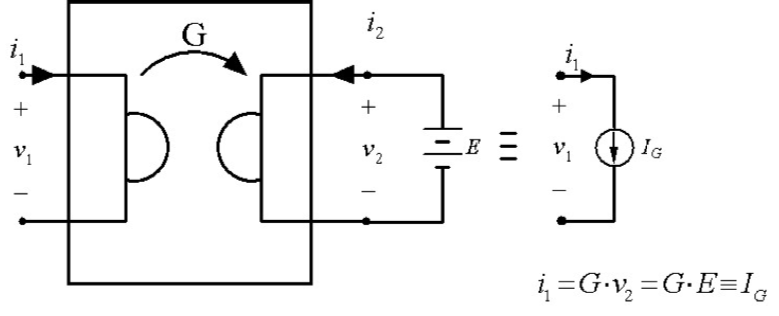
\includegraphics[width=0.7\textwidth, height=4cm]{../Ex2/Resources/ej2_gyrator_prop3.png}
            \caption{Propiedad de inversión corriente - voltaje}
            \label{ej2_gyrator_prop3}
            \end{figure}
    

\end{enumerate}


\section{\textit{Gyrator} como inductor}

Como se vio anteriormente, las propiedades del \textit{Gyrator} hacen posible simular un inductor con un capacitor. El objetivo de esta sección es realizar un circuito que simule un inductor para poder utilizarlo en el armado de filtros activos. 
En la Figura \ref{ej2_inductor_model} se puede ver el modelo del inductor. Si se define su impedancia de entrada como $Z_{in}$:

\begin{equation} Z_{in} = R_L + sL \label{ej2_ecua_inductor}\end{equation}

\begin{figure}[h!]                                                       
    \centering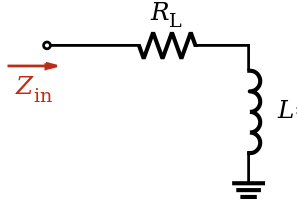
\includegraphics[width=0.4\textwidth, height=4cm]{../Ex2/Resources/ej2_inductor_model.png}
    \caption{Modelo del inductor}
    \label{ej2_inductor_model}
    \end{figure}


\begin{figure}[h!]                                                       
    \centering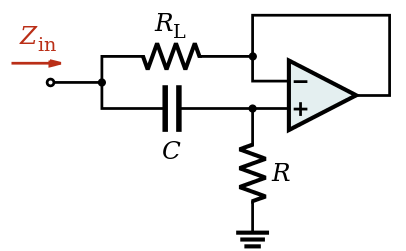
\includegraphics[width=0.4\textwidth, height=4cm]{../Ex2/Resources/ej2_gyrator_inductor.png}
    \caption{\textit{Gyrator} equivalente a un inductor}
    \label{ej2_gyrator_inductor}
    \end{figure}



Se propone el circuito de la Figura \ref{ej2_gyrator_inductor}. Este es un \textit{Gyrator} que simula inductor. Esta compuesto por un amplificador operacional (en configuración de \textit{Buffer}), resistencias y capacitores. A continuación se calcula su impedancia de entrada para analizar 
bajo que condiciones se puede considerar al circuito como un inductor. Es decir, lograr que el circuito \ref{ej2_gyrator_inductor} se parezca al circuito \ref{ej2_inductor_model}.

Se comienza con la ecuación del amplificador operacional. Si se considera que $V_{out}$ es la tensión de salida del \textit{Buffer}
\begin{displaymath} V_{out} = A_{vol} (V^+ - V^-) \end{displaymath}
\begin{displaymath} V^- = A_{vol} (V^+ - V^-) \end{displaymath}
\begin{displaymath} V^- = V^+\frac{A_{vol}}{1+A_{vol}} \end{displaymath}  
\begin{displaymath}  si \hspace{2mm} K = \frac{A_{vol}}{1+A_{vol}} \end{displaymath} 

\begin{equation} V^- = V^+K \label{ej2_ecua_aux_1}\end{equation}


Nótese que se considera al amplificador operacional sin corrientes de bias ni tensiones de offset.

Se continua con la tensión de entrada al circuito, $V_{in}$. Por divisor de tensión, $V_{in}$ es:

\begin{equation} V^+ = V_{in} \frac{R}{R+\frac{1}{sC}} \label{ej2_ecua_aux_2}\end{equation}

Si se juntan (\ref{ej2_ecua_aux_1}) y (\ref{ej2_ecua_aux_2}):
\begin{displaymath} V^- = V_{in} \frac{R}{R+\frac{1}{sC}} K \end{displaymath}

Si se define $I_1$ como la corriente que circula por $R_L$:

\begin{displaymath} I_1 = \frac{V_{in} - V^-}{R_L} \end{displaymath}

\begin{displaymath} I_1 = \frac{V_{in}}{R_L}[1-\frac{R_1}{R_1 + \frac{1}{sC}}K] \end{displaymath}

Si se define $I_2$ como la corriente que circula por $R$ y $C$:    

\begin{displaymath} I_2 = \frac{V_{in} - 0}{R + \frac{1}{sC}} \end{displaymath}

Si se define $I_{in}$ como la corriente entrante al circuito:
\begin{displaymath} I_{in} = I_1 + I_2 \end{displaymath}
\begin{displaymath} I_{in} = \frac{V_{in}}{R_L}[1-\frac{R_1}{R_1 + \frac{1}{sC}}K]  + \frac{V_{in}}{R + \frac{1}{sC}}  \end{displaymath}
\begin{displaymath} I_{in} = V_{in}[\frac{R + \frac{1}{sC} - RK + R_L}{R_L (R + \frac{1}{sC})}]  \end{displaymath}
\begin{displaymath} Z_{in} = \frac{V_{in}}{I_{in}} = \frac{R_L (R + \frac{1}{sC})}{R + \frac{1}{sC} - RK + R_L }  \end{displaymath}

\begin{equation} Z_{in} = \frac{sC R_L R + R_L}{sCR - RsCK +sCR_L + 1} \label{ej2_ecua_impedancia_entrada}\end{equation}

Al tener la expresión de la impedancia de entrada del circuito en la ecuación (\ref{ej2_ecua_impedancia_entrada}) es posible definir condiciones para lograr que se parezca a la ecuación (\ref{ej2_ecua_inductor}).
Para lograrlo se vuelve a la ecuación (\ref{ej2_ecua_aux_1}). Si se considera el modelo del polo dominante, $K$ sufre modificaciones:

\begin{displaymath} V^- = V^+ K = V^+\frac{A_{vol}}{1+A_{vol}} \end{displaymath}  
\begin{displaymath} V^- = V^+\frac{[\frac{A_{0}}{1+\frac{s}{\omega_P}}]}{1+[\frac{A_{0}}{1+\frac{s}{\omega_P}}]} \end{displaymath}  
\begin{displaymath} V^- = V^+ \frac{A_0}{1+ \frac{s}{\omega_P} + A_0} \end{displaymath}  
\begin{displaymath} V^- = V^+ \frac{A_0}{[1+ A_0]} \frac{1}{1+ \frac{s}{\omega_P [1 + A_0]}} \end{displaymath}  
\begin{displaymath} si \hspace{1mm} A_0 + 1 \simeq A_0 \end{displaymath}  
\begin{displaymath} V^- = V^+ \frac{1}{1 + \frac{s}{A_0 \omega_P}}  \end{displaymath}  
\begin{displaymath} A_0 \omega_P = BWP \hspace{1mm}(Band\hspace{1mm}Width\hspace{1mm}Product) \end{displaymath}  
\begin{displaymath} V^- = V^+ \frac{1}{1 + \frac{s}{BWP}}  \end{displaymath}  
Luego, el nuevo $K$ es:
\begin{displaymath} K = \frac{1}{1 + \frac{s}{BWP}}  \end{displaymath}  
Como se puede observar, $K$ es asemeja a la trasferencia de un pasabajos con frecuencia de corte en $f_c = \frac{BWP}{2\pi}$. Luego, si se trabaja en frecuencias menores a $f_c$ se puede tomar $K=1$. Como criterio se toma que esta frecuencia de trabajo $f$ sea 
a lo sumo igual a la frecuencia una decada antes de $f_c$. Entonces:

\begin{equation} f < \frac{BWP}{10 *2\pi} \label{ej2_ecua_condicion_1}\end{equation}

Nótese que, como $BWP$ es del orden de los $MHz$, $K$ comienza a obtener importancia cuando se trabaja en frecuencias del orden de los $MHz$. Consecuentemente, cuando se trabaje en este orden de frecuencias, se debe considerar el efecto del polo dominante.  


Volviendo a (\ref{ej2_ecua_impedancia_entrada}), si se impone el nuevo $K$ la ecuación queda:
\begin{displaymath} Z_{in} = \frac{sC R_L R + R_L}{sCR_L + 1} \end{displaymath}  
\begin{equation} Z_{in} = \frac{R_L [sCR + 1]}{sCR_L + 1} \label{equ:ej2_impedancia_gyrator} \end{equation}  
    
Algo muy interesante para observar es que, al imponer que $K=1$ es indistinto si se conecta el buffer a la entrada inversora o a la entrada no inversora. 


Al tener la expresión de la impedancia de entrada (\ref{equ:ej2_impedancia_gyrator}) se puede ver que la misma cuenta con un cero en $\frac{1}{CR}$ y un polo en $\frac{1}{R_L C}$. Para una mayor comprensión, se simula el circuito del \textit{Gyrator}. En la Figura \ref{ej2_sim_inductor} se puede ver una simulación dándole los siguientes valores a los componentes: 

\begin{table}[h!]
    \centering
    \begin{tabular}{@{}cc@{}}
    \toprule
    Componente   & Valor \\ \midrule
    \text{C}   & 100nF \\
    \text{$R$}   & $1k\Omega$     \\
    \text{$R_L$} & $10\Omega$    \\ 

    \end{tabular}
    \caption{Componentes del \textit{Gyrator}}
    \label{ej2_sim_inductor}
    \end{table}
    

\begin{figure}[h!]                                                       
    \centering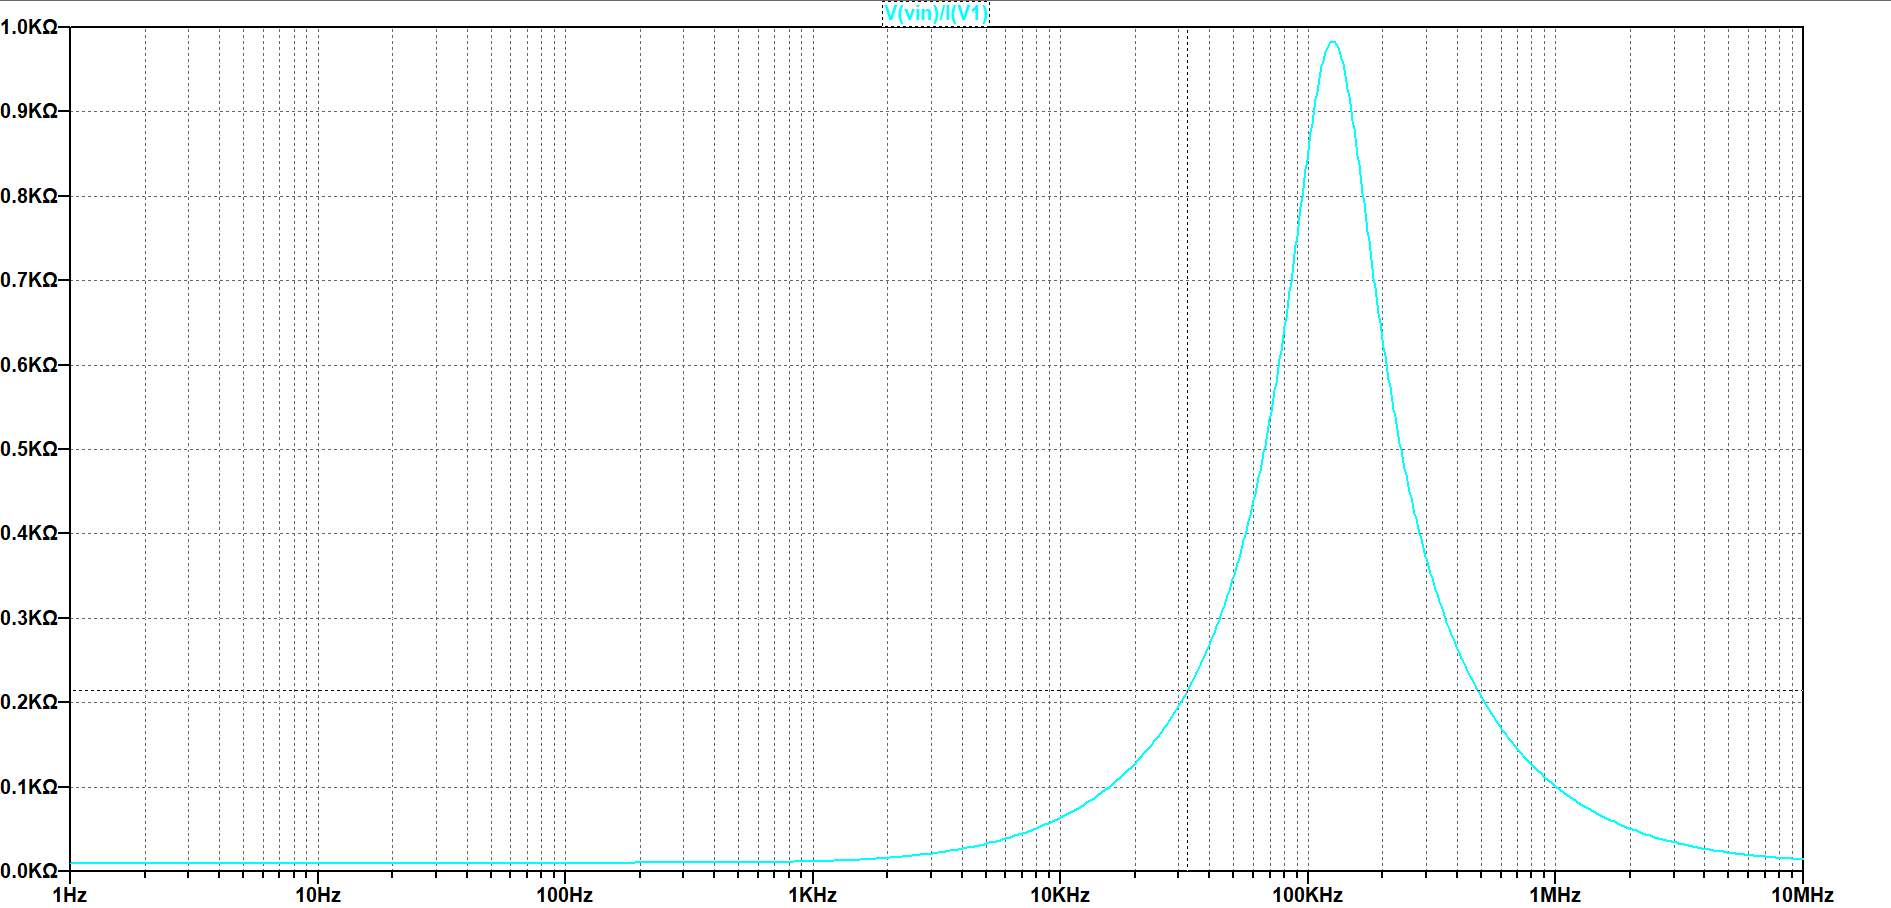
\includegraphics[width=0.9\textwidth, height=9cm]{../Ex2/Resources/ej2_gyrator_sim.png}
    \caption{Simulación de \textit{Gyrator} }
    \label{ej2_sim_inductor}
    \end{figure}

Esta ultima figura muestra el comportamiento de un pasa banda. Sin embargo, la parte de interés es cuando se comporta como una bobina. Esta zona de interés es justamente antes de que el polo entre en acción. Habiendo dicho esto, lo ideal seria que el polo (osea el denominador)
de la impedancia no existiera. Si se cumple esta condición, la impedancia seria idéntica al modelo del inductor (\ref{ej2_ecua_inductor}). Luego para que el denominador sea igual a 1, se debe cumplir que $scR_L << 1 $. 

Se impone una nueva condición:

\begin{displaymath} sCR_L << 1 \end{displaymath}  
\begin{displaymath} sCR_L < 1 * 0,05 \end{displaymath}  
\begin{displaymath} f 2\pi CR_L < 1 * 0,05 \end{displaymath} 
\begin{equation} f < \frac{0.1}{2 \pi R_L C} \label{ej2_ecua_condicion_2} \end{equation}

Esta ultima condición implica que el termino $sCR_L$ debe ser despreciable frente a la unidad para todo el rango de frecuencias en que se desea que el \textit{Gyrator} funcione como (\ref{ej2_ecua_inductor}). Entonces, se puede imponer como regla que $R_L$ debe ser de valor chico (del orden de los $\Omega$) y que $C$ debe ser de valor de, por ejemplo, del orden de los nano Faradios. Como se vera mas adelante, si se utiliza $C = 100n$ y $R_L = 10\Omega$, se pude obtener un rango de trabajo considerable. 

Todas las ecuaciones obtenidas son validas siempre y cuando se cumplan las condiciones anteriormente mencionadas (\ref{ej2_ecua_condicion_1}) y (\ref{ej2_ecua_condicion_2}). Ademas, se debe tener en cuenta que se hizo todo el análisis considerando que el \textit{Gyrator} este conectado a tierra por lo que esta es una nueva condición para tener en cuenta. 

Para concluir se puede hacer una síntesis de los valores hallados:

Si se trabaja a una frecuencia menor a $f = \frac{BWP}{10 *2\pi}$ y el termino $sCR_L$ se mantiene despreciable frente a la unidad, la impedancia del \textit{Gyrator} es:

\begin{displaymath} Z_{in} = R_L + sC R_L R \end{displaymath}

Donde, 

\begin{equation} L = C R_L R \label{ej2_ecua_gyrator_3}\end{equation}
%\begin{equation} R = R_{\textit{Gyrator}} = \frac{L}{C R_L} \label{ej2_ecua_gyrator_4}\end{equation}    
%\begin{equation} |Z_{in}| = \sqrt{(2\pi CR_LR)^2 + R_L^2} \label{ej2_ecua_gyrator_4}\end{equation}
%\begin{equation} Z_{in} = \arctan(2\pi CR)\label{ej2_ecua_gyrator_4}\end{equation}    




\section {Diseño de filtros activos con \textit{Gyrator}}
En esta sección se analizan y diseñan cuatro filtros activos de segundo orden con \textit{Gyrators}. En todos los filtros se considera que el amplificador operacional tiene $r_d = \infty$ y $r_0 = 0$. Ademas, se considera que el amplificador no tiene
ni corrientes de bias ni tensiones de offset.  


\subsection{Filtro pasa altos}
El objetivo de esta sección es diseñar un filtro pasa altos que involucre el uso de un \textit{Gyrator}. El mismo debe cumplir cierta plantilla por lo que se debe estudiar la función transferencia y analizar principalmente el comportamiento del \textit{Gyrator}. 


\subsubsection{Plantilla}
La plantilla para el filtro pasa altos es la siguiente:

\begin{enumerate}
	\item Ganancia unitaria cuando $f \rightarrow \infty$
	\item Ganancia mayor a $-3dB$ para $f>f_p = 14k$
	\item Ganancia menor a $-10dB$ para $f<f_a = 4k$
	\item Ganancia nunca superior a $0dB$  
\end{enumerate}

Haciendo un análisis previo de estas condiciones, se puede decir que que la mas critica es la condición numero 4. Esta condición impone que el filtro no tenga ningún sobrepico por lo que se deben tener ciertas precauciones. Dichas precauciones se debaten mas adelante. En cuanto a la condición 1, la misma exhibe gran complejidad. Como se vio en la sección de estudio del \textit{Gyrator}, el mismo tiene un rango de frecuencias para la cual se comporta como un inductor. Entonces, se puede decir de ante mano que para cierta frecuencia (cuando el \textit{Gyrator} deje de ser un inductor) el circuito pase a comportarse de manera indeseada y no se podrá cumplir la condición 1. Todo esto quedara mas claro al avanzar en el diseño del filtro. 

\subsubsection{Funcion transferencia y circuito de segundo orden}

Un circuito clásico de segundo orden que representa un pasa altos es un RCL con salida en la inductancia. En la Figura \ref{ej2_filto_HP} se puede ver dicho circuito. 
%Grafico clasico RCL
\begin{figure}[h!]                                                       
    \centering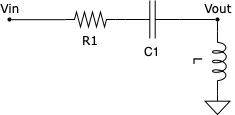
\includegraphics[width=5cm, height=3cm]{../Ex2/Resources/ej2_hp.png}
    \caption{Pasa altos de segundo orden}
    \label{ej2_filto_HP}
    \end{figure}


La función transferencia de este circuito es:

\begin{displaymath} H(j\omega)= H_{0HP} H_{HP} \end{displaymath}  
Donde $H_{0HP}$ es la ganancia en altas frecuencias. Por la condición 1, $H_{0HP} = 1$. Luego:   

\begin{equation} H(j\omega) = \frac{-(\frac{\omega}{\omega_0})^{2}}{1 - (\frac{\omega}{\omega_0})^{2} + (\frac{j\omega}{\omega_0})\frac{1}{Q}} \label{equ:trans_clasica_hp}\end{equation}  

Donde $Q$ es el factor de calidad y $\omega_0$ es la frecuencia de corte.      
Al tener conocimiento de la función transferencia $H(jw)$ es posible proponer un circuito para tratar de obtener una nueva función transferencia que se asemeje lo mas posible a $H(jw)$. 

\subsubsection{Circuito propuesto}
Teniendo en mente el circuito de la Figura \ref{ej2_filto_HP}, se propone un nuevo circuito reemplazando el inductor por un \textit{Gyrator}. El circuito resultante se muestra en la Figura \ref{fig:ej2_HP_propuesto}. 

%Circuito propuesto
\begin{figure}[!]                                                       
    \centering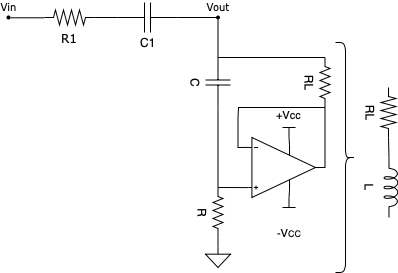
\includegraphics[width=0.4\textwidth, height=4cm]{../Ex2/Resources/ej2_hp_gyrator.png}
    \caption{Circuito propuesto}
    \label{fig:ej2_HP_propuesto}
    \end{figure}

Nótese que la impedancia del \textit{Gyrator} es $Z = R_L + sR_L R C$ (si se cumple (\ref{ej2_ecua_condicion_2})) como se vio en la sección anterior. El circuito propuesto tiene la siguiente función transferencia:

\begin{displaymath} H(s)= \frac{V_{out}}{V_{in}} = \frac{R_L + sL}{(R_1 + R_L) +sL + \frac{1}{sC_1}} \end{displaymath}  
\begin{displaymath} H(s)= \frac{[R_L + sL]sC_1}{[R_1 + R_L]sC_1 +s^2LC_1 + 1} \end{displaymath}
\begin{displaymath} H(s)= \frac{s^2CR_LRC_1 + sC_1R_L}{s^2[CR_LRC_1] + s[R_1 + R_L]C_1 + 1} \end{displaymath}

Donde:

\begin{displaymath} \omega_0^2= \frac{1}{CR_LRC_1} \end{displaymath}  
\begin{displaymath} \frac{1}{\omega_0 Q}= (R_1 + R_L) C_1 \end{displaymath}  


Estas expresiones permiten proseguir en la selección de componentes. 


\subsubsection{Diseño del circuito}

Según la plantilla de este filtro, la frecuencia de corte se ubica en $f = 14kHz$. Entonces, $w_0 = 2\pi 14$. Ademas, la plantilla prohíbe tener una ganancia mayor a $0 dB$ para cualquier frecuencia. Esto implica que no pude haber un sobre pico para ninguna frecuencia. Luego, como el parámetro $Q$ es el responsable de que halla sobrepicos en este tipo de filtros, se define  $Q=\frac{1}{\sqrt{2}}$. Dicho valor de $Q$ es el mas grande que puede adquirir antes de que halla sobrepico. Entonces, se asegura que la ganancia nunca supere los $0dB$.  


Ademas se imponen se impone que $R_L = 10 \Omega$ y que $ C = 100nF$ ya que de esta manera se obtiene un buen rango para el cual el \textit{Gyrator} funciona como inductor (se cumple la condición \ref{ej2_ecua_gyrator_2}). Este tema se analiza con mas profundidad en la sección \textit{Simulación y análisis}.

Por ultimo, se define $C_1 = C$ por el simple hecho que simplifica notablemente las expresiones. 

Gracias a todas estas definiciones se pueden obtener dos expresiones para $R$ y $R_1$ y sus valores.  

Luego:

\begin{displaymath} R = \frac{1}{C^2 R_L \omega_0^2} = 1292.36 \Omega \end{displaymath}  
\begin{displaymath} R_1 = \frac{1}{\omega_0 Q C} - 10 = 150.77 \Omega \end{displaymath}  

Si $R$ y $R_1$ adquieren estos valores, se cumplen las condiciones de la plantilla. 

También es de particular interés ver como es afectada la función transferencia bajo estas definiciones:

\begin{displaymath} H(s)= \frac{s^2 10 C ^2 R + sC10}{s^2[C^2 10 R] + s[R_1 + 10]C + 1} \end{displaymath}

Nótese a primera vista la función trasferencia no es exactamente igual a la función transferencia del pasa altos clásica (\ref{equ:trans_clasica_hp}). Sin embargo, si se evaluá a la función con los valores definidos, el termino $sC10$ del numerador es $j2\pi * 1\mathrm{e}{-17}$. Este termino es prácticamente despreciable frente a $s^2 10 C^2 R_L$  por lo que la función trasferencia resulta ser:


\begin{displaymath} H(s)= \frac{s^2 1.5\mathrm{e}{-10}}{s^2[1.5\mathrm{e}{-10}] + s[1.6\mathrm{e}{-5}] + 1} \end{displaymath}


Como no existen los valores comerciales de resistencias $1292.36 \Omega$ y $150.77 \Omega$, estos se redondean para poder realizar el circuito. En la Tabla  \ref{tab:hp_components} se enumeran los componentes utilizados. 

\begin{table}[h!]
    \centering
    \begin{tabular}{@{}cc@{}}
    \toprule
    Componente   & Valor \\ \midrule
    \text{C}   & 100nF \\
    \text{$C_1$}   & 100nF \\
    \text{R}   & $1.5k\Omega$     \\
    \text{$R_L$} & $10\Omega$    \\ 
    \text{$R_1$} & $150\Omega$    \\ \bottomrule
    \end{tabular}
    \caption{Componentes del circuito propuesto}
    \label{tab:hp_components}
    \end{table}

Como se explico anteriormente, el objetivo es realizar cuatro filtros. Se decide, realizar los mismos en el mismo PCB y utilizando el mismo integrado. Dicho integrado es el $TL 084$ que, gracias a la \textit{datasheet} tiene un $BPW$ de $2.5MHz$. Se brinda mas información del PCB final en la sección \textit{Diseño PCB}. Al tener dicho $BPW$, y teniendo en cuenta la condición \ref{ej2_ecua_condicion_1} se debe trabajar a una frecuencia inferior a $40kHz$ para que no se consideren los efectos del polo dominante. 

Antes de continuar con la medición se realiza una simulación montecarlo para evaluar el comportamiento del circuito bajo distintos valores de componentes. Como se vera en la sección \textit{Diseño PCB}
se utilizan todos componentes de montaje superficial con tolerancias $1\%$. El resultado de la simulación se ve en la Figura \ref{fig:monte}. 

\begin{figure}[h!]                                                       
    \centering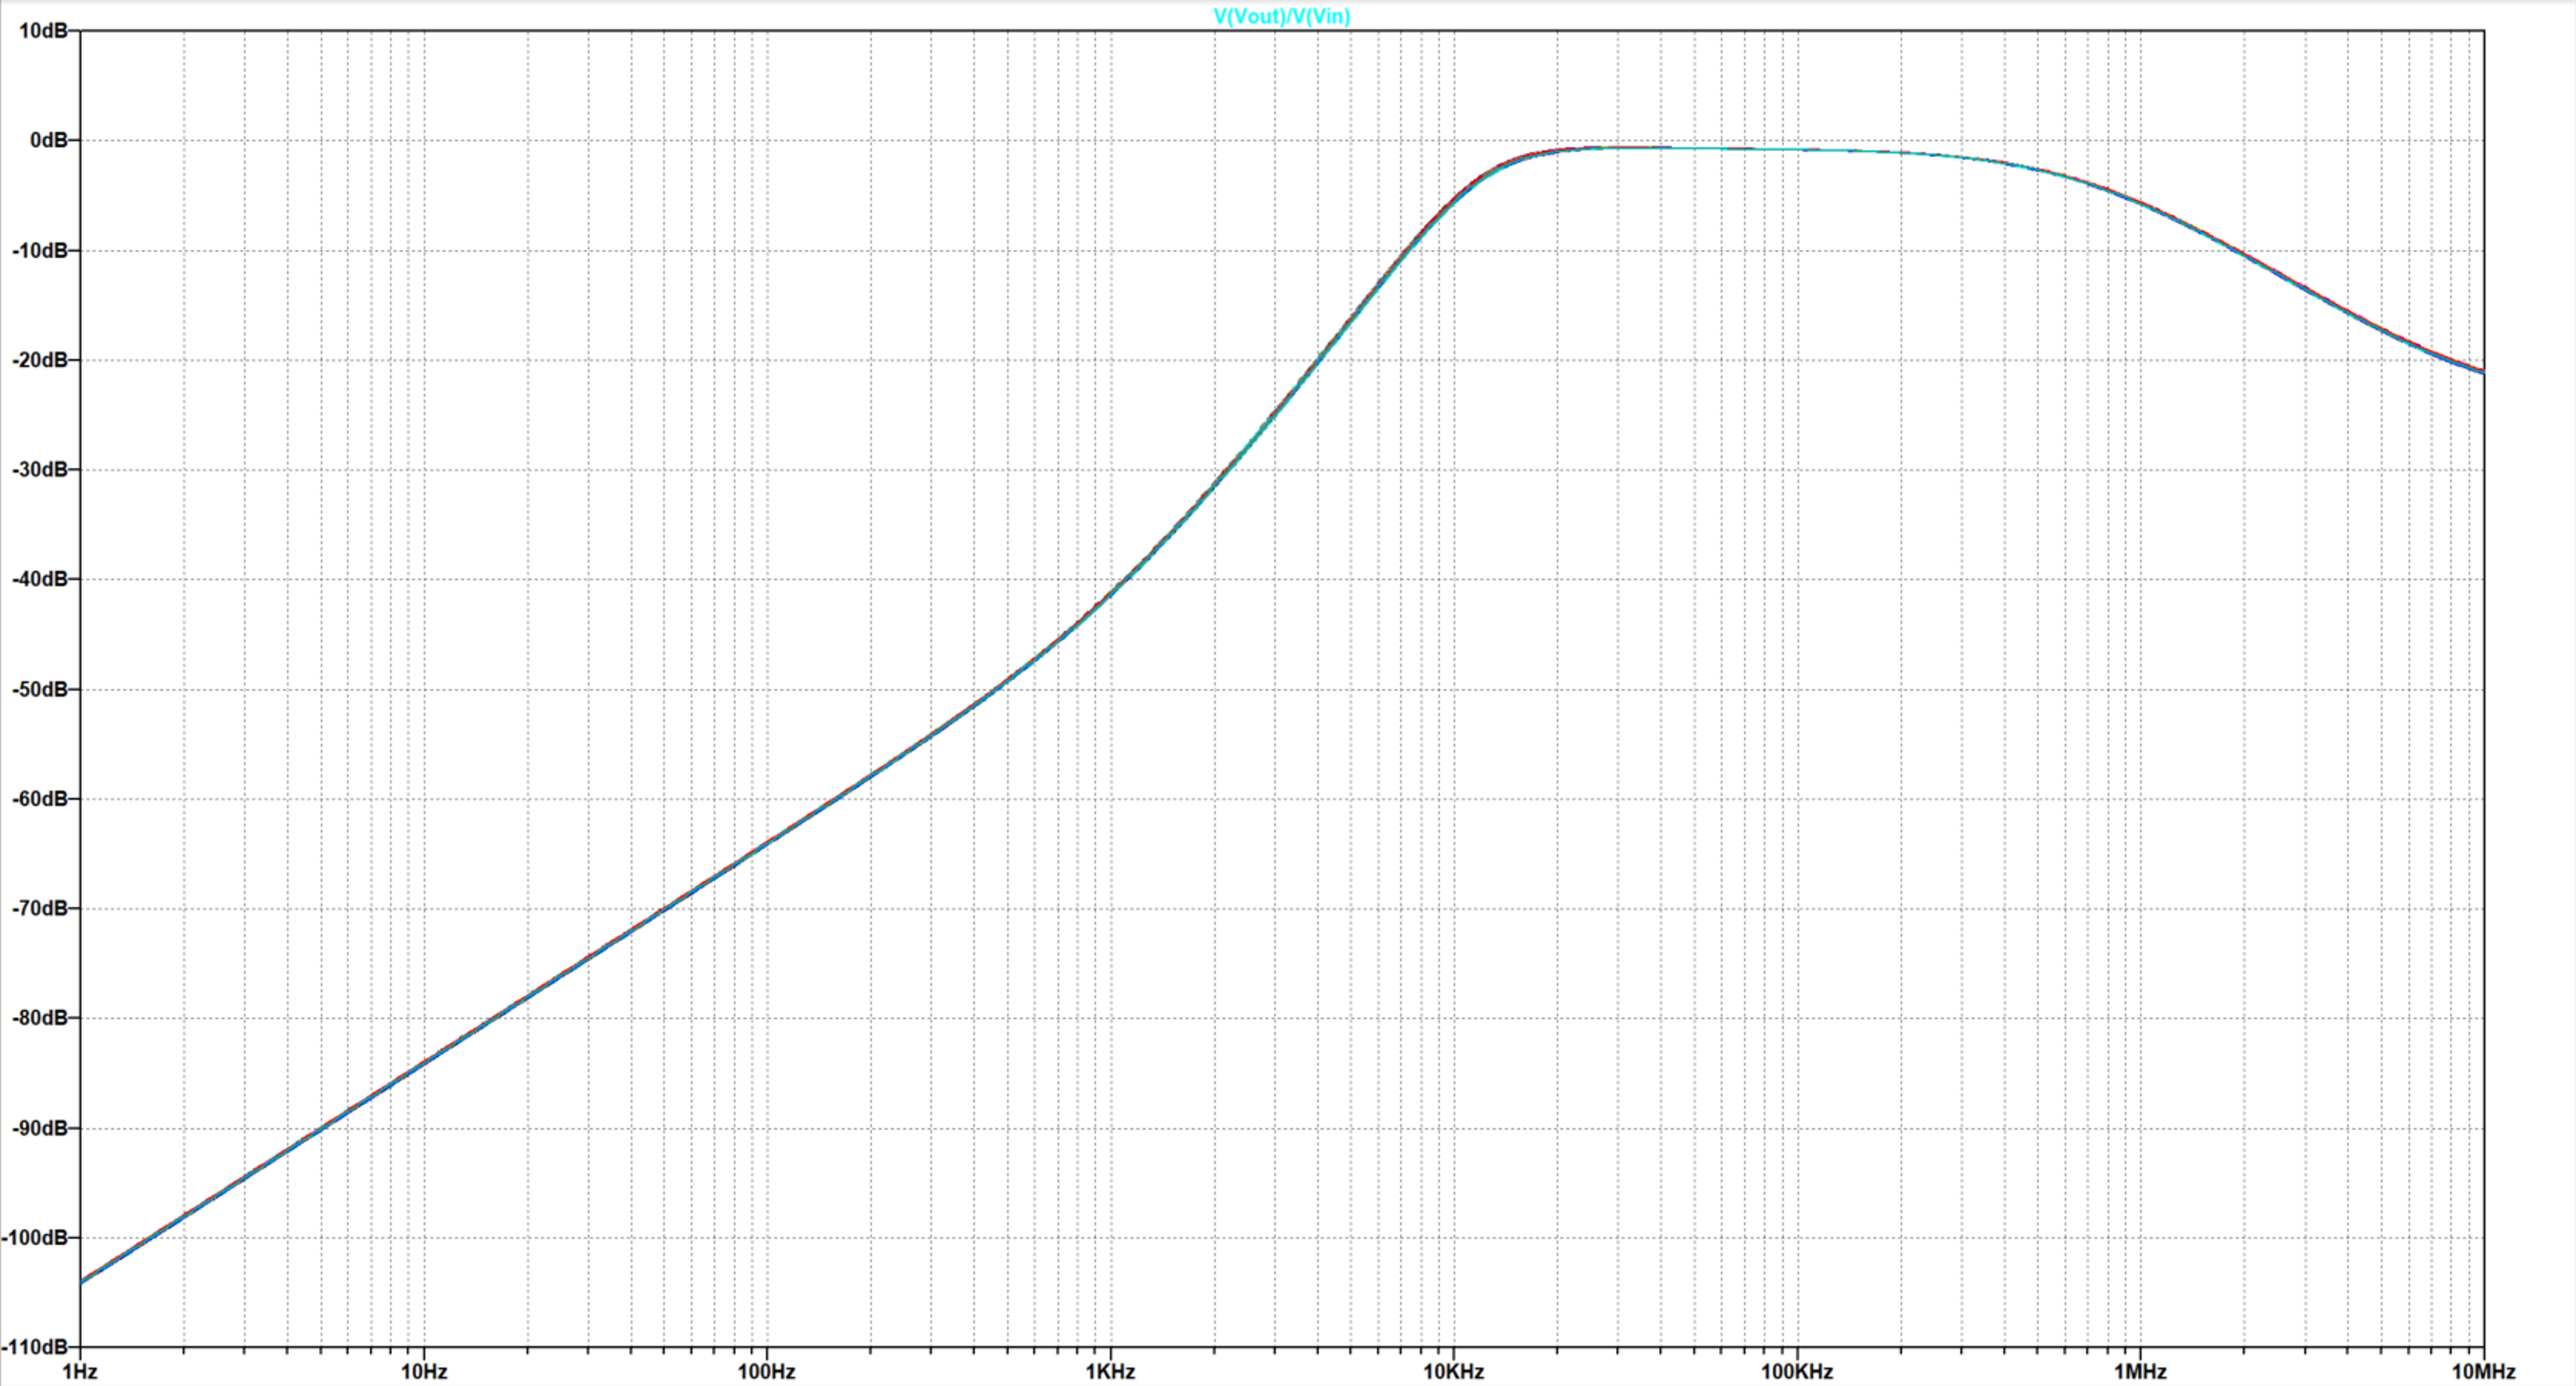
\includegraphics[width=0.9\textwidth, height=7cm]{../Ex2/Resources/ej2_montecarlo.png}
    \caption{Simulación de montecarlo}
    \label{fig:monte}
    \end{figure}
    
La simulación muestra una variación prácticamente imperceptible ya que las tolerancias son muy pequeñas. Se concluye que no se debe corregir los componentes. Esta simulación solo se realiza para este filtro ya que no aporta al análisis de los circuitos. 

\subsubsection{Simulacion y analisis lineal}
Si se simula el circuito propuesto (desde $f = 10 Hz$ a $f = 10MHz$) con los componentes de la Tabla \ref{tab:hf_gyrator_components}, se obtiene el gráfico de la Figura \ref{ej2_hp_sim}.

\begin{figure}[h!]                                                       
    \centering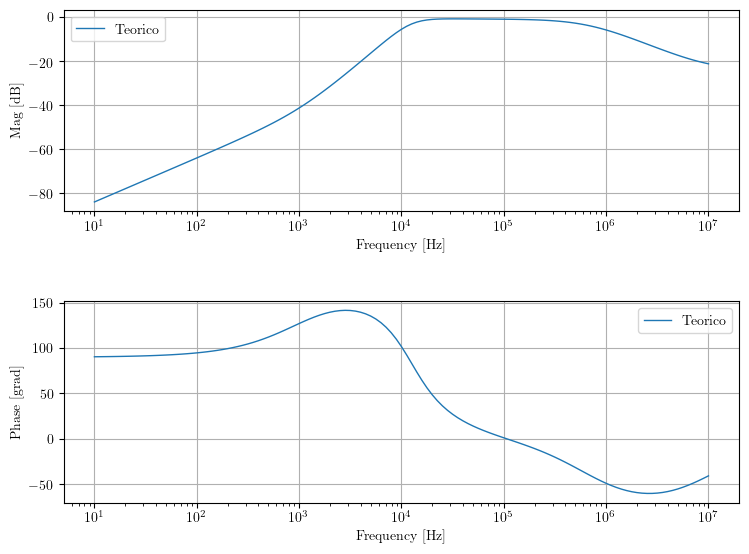
\includegraphics[width=0.9\textwidth, height=9cm]{../Ex2/Resources/ej2_hp_sim.png}
    \caption{Simulación del circuito propuesto }
    \label{ej2_hp_sim}
    \end{figure}

Gracias a las herramientas de LTSpice, se detecta que a la frecuencia $f = 14kHz$ hay una atenuación de $2.15 dB$. Si $f > 14kHz$ la ganancia es mayor a $-3dB$. Luego, la condición 2 se cumple. Si $f < 4kHz$, la ganancia es menor $-10dB$ por lo que la condición 3 también se cumple. Ademas, se puede ver que la ganancia nunca supera los $0dB$ por lo que la condición 4 también se cumple. 

Con respecto a la condición 1, se nota en el diagrama de bode que alrededor de $f = 195 kHz$ la atenuación deja de ser $0dB$ y comienza a aumentar. Esto se debe a que estas frecuencias el \textit{Gyrator} deja de comportarse como un inductor. Para un mejor comprendimiento e lo que sucede, se prosigue a realizar un análisis de linealidad. Gracias a este análisis se puede determinar en que frecuencias el \textit{Gyrator} adquiere la impedancia deseada (\ref{ej2_inductor_model}). Para comenzar el análisis, se simula el \textit{Gyrator} en LTSpice con los valores de $R$, $R_L$ y $C$ propuestos. El resultado se detalla en la Figura \ref{fig:ej2_HP_gyrator_sim}.

\begin{figure}[h!]                                                       
    \centering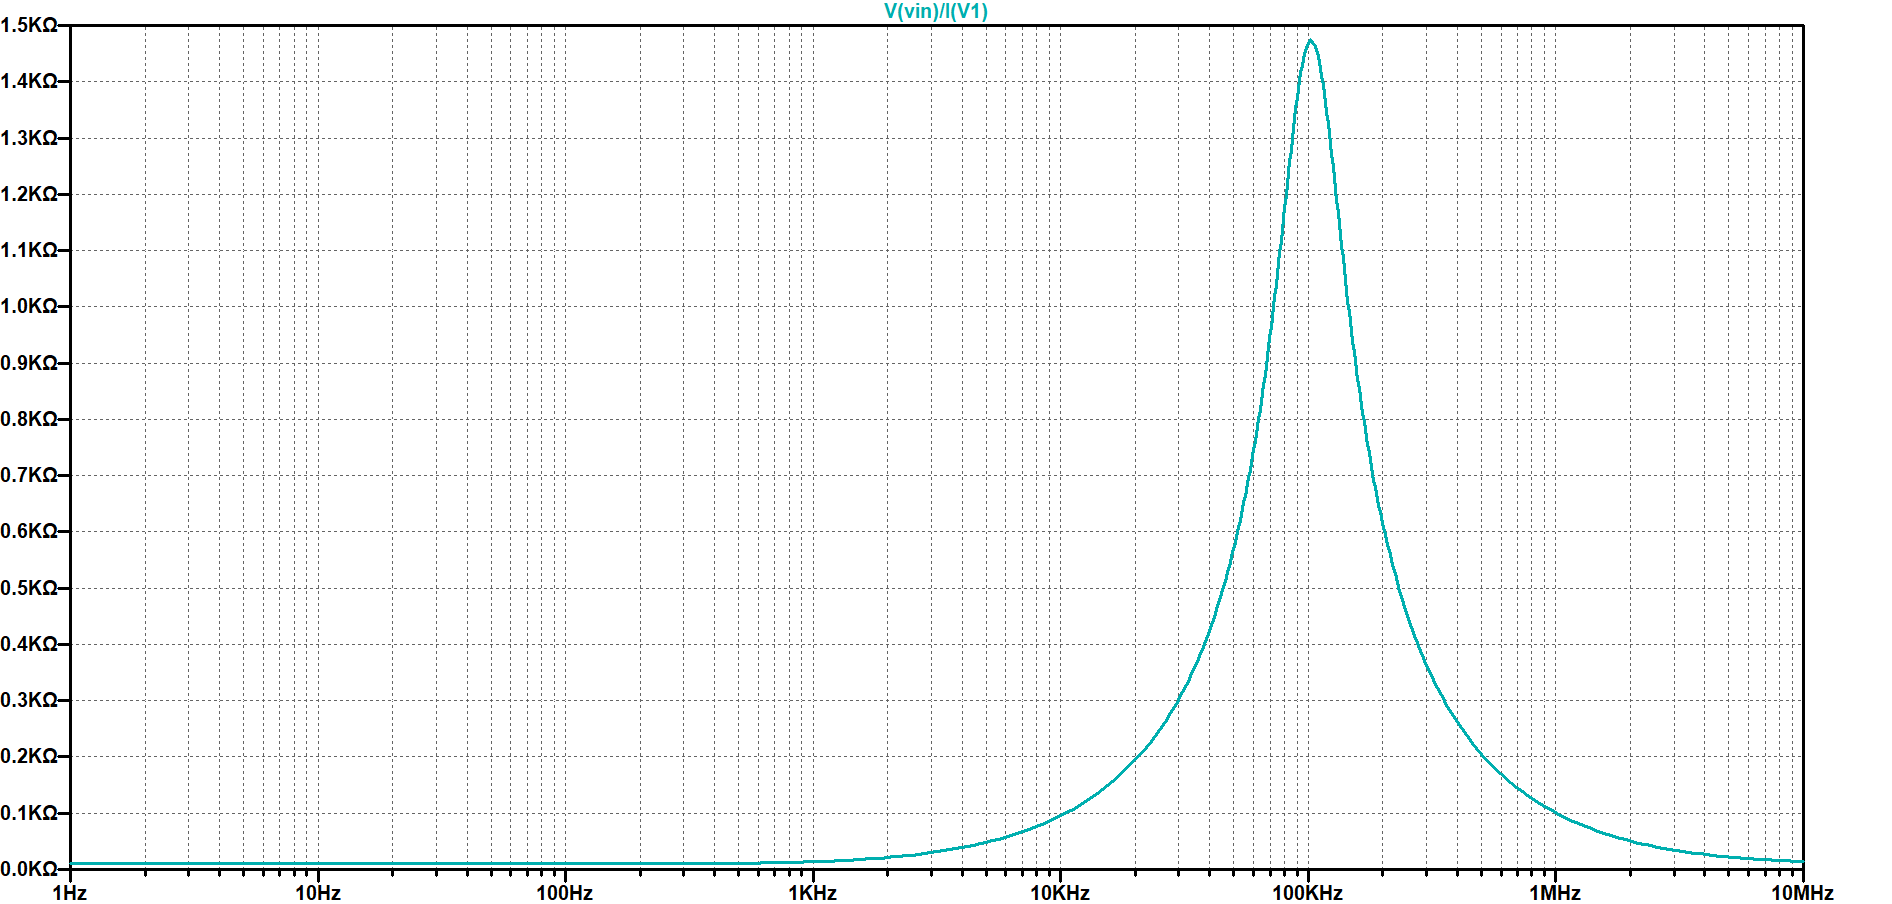
\includegraphics[width=0.9\textwidth, height=7cm]{../Ex2/Resources/ej2_hp_gyrator_sim.png}
    \caption{Simulación del \textit{Gyrator} }
    \label{fig:ej2_HP_gyrator_sim}
    \end{figure}

La simulación detalla como la impedancia del \textit{Gyrator} varia con la frecuencia. Nótese lo siguiente: en el rango de frecuencias que va desde $f = 14 kHz$ a $f = 100 kHz$ la impedancia adopta un comportamiento prácticamente lineal. Esto se debe a que la impedancia del \textit{Gyrator} (\ref{equ:ej2_impedancia_gyrator}) esta bajo la condición \ref{ej2_ecua_condicion_2} y se comporta como la impedancia del modelo de un inductor \ref{ej2_inductor_model}. A hasta la frecuencia de $f=100kHz$ el denominador de (\ref{equ:ej2_impedancia_gyrator}) es despreciable frente a la unidad. Al sobrepasar esta frecuencia provoca un decaimiento en la impedancia. Todo esto explica porque en la simulación del circuito propuesto (Figura \ref{ej2_hp_sim}) la atenuación aumenta a partir de la frecuencia $f = 195 kHz$. 

Cabe destacar que para ambas simulaciones se utilizo un amplificador operacional ideal. Esto hace que no se pueda apreciar los efectos del polo dominante. Los mismos se analizan en la siguiente sección al obtener la medición real del circuito. 

\subsubsection{Medicion y analisis a altas frecuencias}

Al imponer una senoide de $V_{PP} = 3V$ como señal de entrada al circuito en un rango de frecuencias de $[10Hz , 10MHz]$, se obtiene el bode de la Figura \ref{fig:ej2_hp_med_and_sim}. En dicha figura también se superpone la simulación del circuito propuesto.  

\begin{figure}[h!]                                                       
    \centering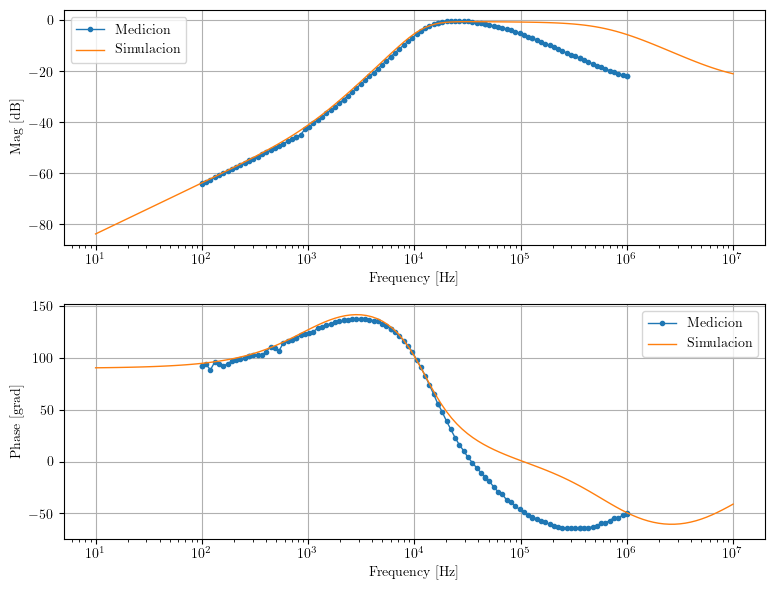
\includegraphics[width=0.9\textwidth, height=7cm]{../Ex2/Resources/ej2_hp_med_and_sim.png}
    \caption{Medición y simulación del circuito propuesto }
    \label{fig:ej2_hp_med_and_sim}
    \end{figure}

Se puede ver que la simulación y la medición se comportan prácticamente igual hasta aproximadamente $40kHz$. A esa frecuencia, se detecta que la medición comienza a atenuar. Esto se debe a la condición (\ref{ej2_ecua_condicion_2}). A estas frecuencias el polo dominante entra en efecto y provoca una atenuación. Esto implica que a altas frecuencias no se puede obtener una ganancia de $0dB$, como propone la plantilla. 



\subsubsection{Conclusion}

En primer lugar, se destaca que se logro hacer un filtro pasa altos sin la utilización de un inductor. Se pudo sustituir dicho componente gracias a la ayuda de la teoría de \textit{Gyrators}. También, se pudo cumplir casi con la totalidad de la plantilla propuesta. En cuanto a la condición de ganancia unitaria para frecuencias infinitas es prácticamente imposible de cumplir ya que como el \textit{Gyrator} esta compuesto de un amplificador operacional, y los amplificadores operacionales ideales no existen, siempre se tendrá el inconveniente del polo dominante. Ademas, como se vio, el \textit{Gyrator} tiene un rango de frecuencias para el cual trabaja como un inductor por lo que inevitablemente a una cierta frecuencia el circuito deja de comportarse como se desea. Se puede concluir que el rango de frecuencias de trabajo de este filtro es hasta $40kHz$. 


\subsection{Pasa Banda}

EL objetivo de esta sección es diseñar un filtro pasa bandas que, como en el caso del pasa altos, involucre el uso de un \textit{Gyrator}. El filtro también debe cumplir cierta plantilla.

\subsubsection{Plantilla}

\begin{enumerate}
	\item Frecuencia de pasabanda de $f = 8kHz$	
\end{enumerate}

Como se puede observar las condiciones de la platilla son muy flexibles ya que no se especifica las frecuencias laterales no la atenuación que estas deben tener. Se prosigue como en el caso anterior. 

\subsubsection{Funcion transferencia y circuito de segundo orden}

Un circuito clásico de segundo orden que representa un pasa bandas es un RCL con el capacitor en paralelo con la bobbina . En la Figura \ref{ej2_filto_BP} se puede ver dicho circuito. 

%Grafico clasico RCL
\begin{figure}[h!]                                                       
    \centering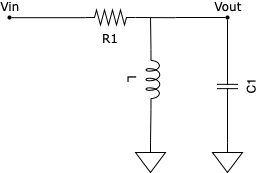
\includegraphics[width=5cm, height=3cm]{../Ex2/Resources/ej2_bp.png}
    \caption{Pasa banda}
    \label{ej2_filto_BP}
    \end{figure}


La función transferencia de este circuito es:


\begin{equation} H(j\omega) = \frac{(\frac{j\omega}{Q\omega_0})}{1 - (\frac{\omega}{\omega_0})^{2} + (\frac{j\omega}{\omega_0})\frac{1}{Q}} \label{equ:trans_clasica_bp}\end{equation}  

Donde $Q$ es el factor de calidad y $\omega_0$ es la frecuencia de corte.      
Al tener conocimiento de la función transferencia $H(jw)$ es posible proponer un circuito para tratar de obtener una nueva función transferencia que se asemeje lo mas posible a $H(jw)$. 

\subsubsection{Circuito propuesto}
Se propone el circuito de la Figura \ref{fig:ej2_BP_propuesto}. 

%Circuito propuesto
\begin{figure}[!]                                                       
    \centering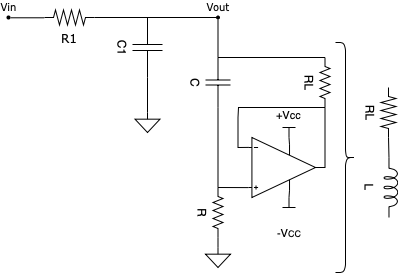
\includegraphics[width=0.4\textwidth, height=4cm]{../Ex2/Resources/ej2_bp_gyrator.png}
    \caption{Circuito propuesto}
    \label{fig:ej2_BP_propuesto}
    \end{figure}

Se puede extraer la siguiente función transferencia:

\begin{displaymath} H(s)= \frac{V_{out}}{V_{in}} = \frac{R_L + sL}{[1+sC R_L + s^2 C L] [R_1 + \frac{R_L + sL}{1 + sCR_L + s^2 C L}]} \end{displaymath}  
\begin{displaymath} H(s)= \frac{\frac{R_L + sL}{[R_1 + R_L]}}{\frac{s^2 C_1 L R_1}{[R_1 + R_L]} + \frac{s C_1 R_L R_1 + L}{R_1 + R_L} +1} \end{displaymath}
\begin{displaymath} H(s)= \frac{\frac{R_L + sCR R_L}{[R_1 + R_L]}}{\frac{s^2 C_1 CR R_L R_1}{[R_1 + R_L]} + \frac{s C_1 R_L R_1 + CR R_L}{R_1 + R_L} +1} \end{displaymath}

Donde:

\begin{displaymath} \omega_0^2= \frac{R_1 + R_L}{CR_LRC_1 R_1} \end{displaymath}  
\begin{displaymath} \frac{1}{\omega_0 Q}= \frac{C_1 R_L R_1 + R_L R C}{R_1 + R_L} \end{displaymath}  





\subsubsection{Diseño del circuito}


Al igual que en el filtro anterior, se seleccionan los componentes. Como se obtuvieron en el filtro anterior muy buenos resultados al definir $R_L = 10 \Omega$ y $ C = 100nF$, se utilizan los mismos valores. En este caso se define $Q = 1$,  $C_1 = C$ y $\omega_0 = 2\pi 8k$. 


Gracias a todas estas definiciones se pueden obtener dos ecuaciones que dependen tanto de  $R$ y $R_1$:.  

Luego:

\begin{displaymath} R = \frac{R_1 + R_L }{C^2 R_L R_1 \omega_0^2} = 4147.26 \Omega \end{displaymath}  
\begin{displaymath} R_1 = \frac{R_L R C - \frac{R_L}{\omega_0 Q}}{\frac{1}{\omega_0 Q} - R_L C} = 208.96 \Omega \end{displaymath} 


Al tener los valores de todos los componentes, se puede formar la Tabla  \ref{tab:bp_gyrator_components} de los componentes utilizados. 

\begin{table}[h!]
    \centering
    \begin{tabular}{@{}cc@{}}
    \toprule
    Componente   & Valor \\ \midrule
    \text{C}   & 100nF \\
    \text{$C_1$}   & 100nF \\
    \text{$R_A$}   & $3.9k\Omega$     \\
    \text{$R_B$}   & $240\Omega$     \\
    \text{$R_L$} & $10\Omega$    \\ 
    \text{$R_1$} & $200\Omega$    \\ \bottomrule
    \end{tabular}
    \caption{Componentes del circuito propuesto}
    \label{tab:bp_gyrator_components}
    \end{table}

    
    
\subsubsection{Simulacion y analisis lineal}
Si se simula el circuito propuesto (desde $f = 1 Hz$ a $f = 10MHz$) con los componentes de la Tabla \ref{tab:bp_gyrator_components}, se obtiene el gráfico de la Figura \ref{ej2_bp_sim}.

\begin{figure}[h!]                                                       
    \centering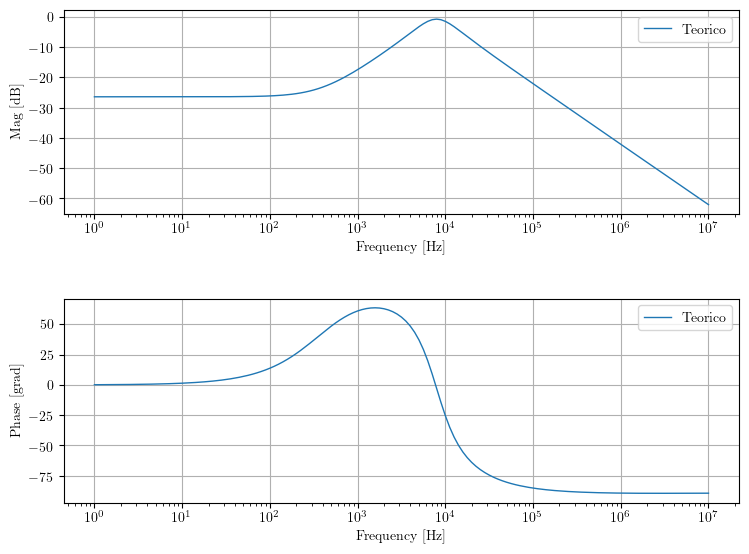
\includegraphics[width=0.9\textwidth, height=9cm]{../Ex2/Resources/ej2_bp_sim.png}
    \caption{Simulación del circuito propuesto }
    \label{ej2_bp_sim}
    \end{figure}

Como se puede ver en la Figura, el bode describe un pasa banda. Se detecta que a la frecuencia $f = 8kHz$ hay una atenuación de $800 mdB$, siendo esta la menor atenuación en todo el rango de frecuencias. Como la plantilla no especifica las frecuencias laterales, es de interés averiguarlas mediante el bode. Las dos frecuencias en las que se detecta una atenuación de $3 dB$ son $f_1 = 5kHz$ y $f_2 = 12.2kHz$. 


Al igual que en la sección anterior, se realiza un análisis lineal. En la Figura \ref{fig:ej2_HP_gyrator_sim} se simula el circuito del \textit{Gyrator} con los correspondientes  $R_A$, $R_B$,  $R_L$ y $C$.



\begin{figure}[h!]                                                       
    \centering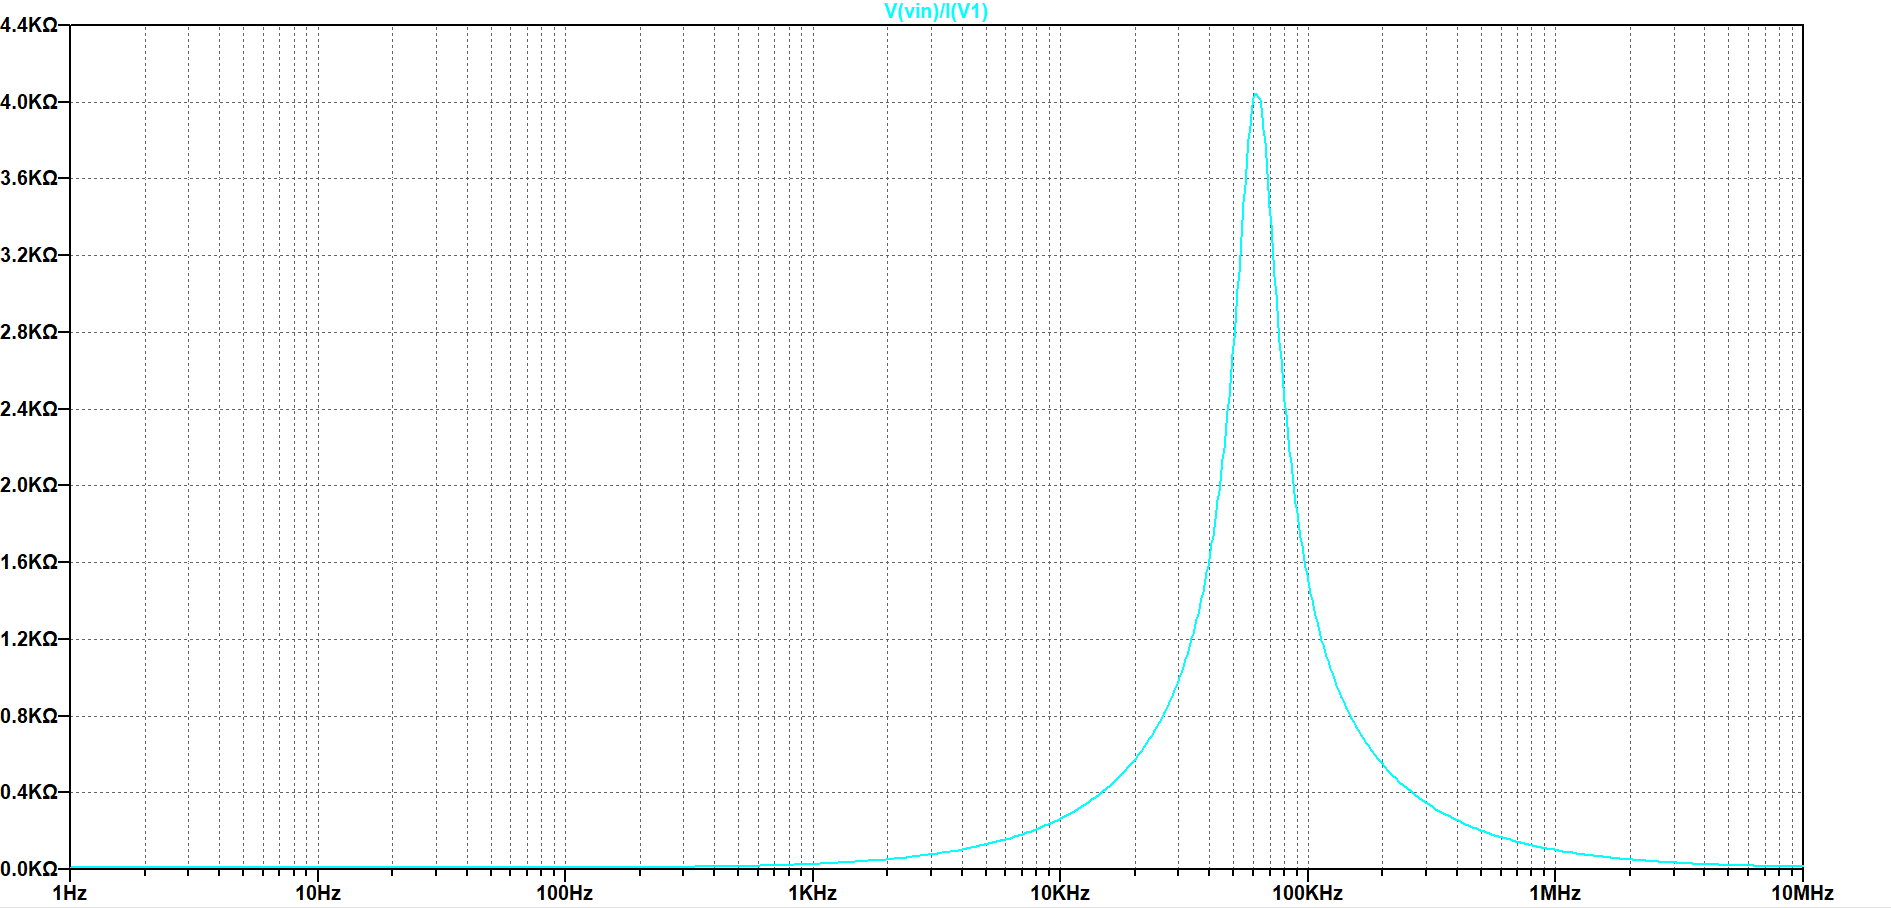
\includegraphics[width=0.9\textwidth, height=7cm]{../Ex2/Resources/ej2_bp_gyrator_sim.png}
    \caption{Simulación del \textit{Gyrator} }
    \label{fig:ej2_BP_gyrator_sim}
    \end{figure}


En la simulación del \textit{Gyrator}, se puede apreciar que la impedancia tiene un comportamiento creciente hasta que llega a una frecuencia aproximada de $f = 62 kHz$. Al sobrepasar esta frecuencia, la impedancia decae abruptamente. Como esto recién sucede a una frecuencia mucho mayor que $f=8kHz$, se puede decir que el \textit{Gyrator} se comporta como un inductor en un rango de frecuencias considerable. 

\subsubsection{Medicion y analisis a altas frecuencias}

Al imponer una senoide de $V_{PP} = 3V$ como señal de entrada al circuito en un rango de frecuencias de $[10Hz , 1MHz]$, se obtiene el bode de la Figura \ref{fig:ej2_hp_sim_y_medicion}. En dicha imagen también se superpone la simulación anteriormente mostrada para poder comparar resultados. A primera vista el resultado es muy bueno. Tanto para bajas, medias y altas frecuencias el circuito propuesto se comporta como en la simulación. Al igual que en la simulación, la frecuencia máxima se da en aproximadamente la misma frecuencia. Otra cosa para notar es el polo dominante. En este caso, el filtro se beneficia de el ya que a frecuencias altas tiende a atenuar las señales. Esto implica que la condición (\ref{ej2_ecua_condicion_1}) se puede dejar de lado.  

\begin{figure}[h!]                                                       
    \centering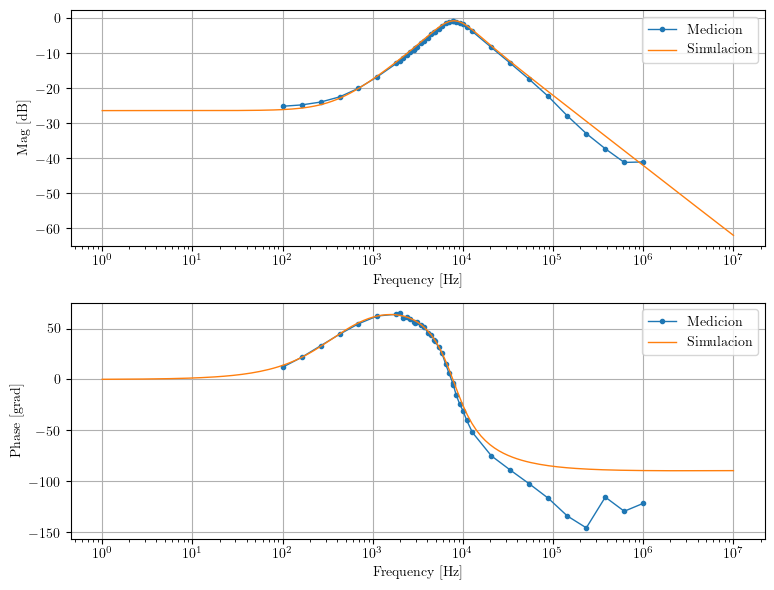
\includegraphics[width=0.9\textwidth, height=9cm]{../Ex2/Resources/ej2_bp_med_and_sim.png}
    \caption{Bode de medición y simulación}
    \label{fig:ej2_hp_sim_y_medicion}
    \end{figure}

\subsubsection{Conclusion}

Se logro utilizar un \textit{Gyrator} para crear un filtro pasa banda. Como la plantilla para este filtro es sencilla y flexible se logro crear el filtro sin mayor inconvenientes. El circuito propuesto resulto como se esperaba. La medición y la simulación se asemejan. Ambas, se comportan prácticamente igual en todo el rango de frecuencias e incluso se utiliza el factor del polo dominante a favor. Finalmente, se puede decir que este filtro funciona para un amplio rango de frecuencias que va desde bajas frecuencias ($10Hz$) hasta $10Mhz$. 







%La funcion trasferencia resulta:
%\begin{displaymath} H(s)= \frac{V_{out}}{V_{in}} = \frac{R_L + sL}{(R_1 + R_L) +sL + \frac{1}{sC_1}} \end{displaymath}  
%\begin{displaymath} H(s)= \frac{[R_L + sL]sC_1}{[R_1 + R_L]sC_1 +s^2LC_1 + 1} \end{displaymath}
%\begin{displaymath} H(s)= \frac{s^2CR_LRC_1 + sC_1R_L}{s^2[CR_LRC_1] + s[R_1 + R_L]C_1 + 1} \end{displaymath}
%Si se impone la siguiente condicion para simplificar las cuentas:
%\begin{displaymath} R_L = R \end{displaymath}
%\begin{displaymath} C_1 = C \end{displaymath}
%\begin{displaymath} H(s)= \frac{s^2 [CR_L]^2 + sCR_L}{s^2[CR_L]^2 + s[R_1 + R_L]C + 1} \end{displaymath}
%Si bien la funcion trasferencia no es exactamente igual a la funcion trasferencia clasica de un pasa altos de segundo orden, la funcion hallada sigue 
%siendo un filtro de segundo orden. 

%De la funcion trasferencia se puede obtener la frecuencia de corte $\omega_0$:

%\begin{displaymath} \omega_0 = \frac{1}{C R_L}  \end{displaymath}

%Ademas, se puede obtener una expresion para $Q$: 
%\begin{displaymath} \frac{1}{\omega_0 Q} = C_1 [R_1 + R_L]  \end{displaymath}
%\begin{displaymath} \frac{1}{\omega_0 Q} = [\frac{R_1}{R_L} + 1]  \end{displaymath}

%La condición 4 impide que halla un sobre pico. Luego, $Q$ debe tener un valor menor a $1$. Como el $Q$ mas grande antes del sobre pico es $Q=\frac{1}{\sqrt{2}}$. Entonces:
%\begin{displaymath} \frac{1}{\sqrt{2}} < C_1 [\frac{R_1}{R_L} + 1]   \end{displaymath}
%\begin{displaymath} -1 + \sqrt{2} < \frac{R_1}{R_L}  \end{displaymath}



\subsection{Rechaza banda}

En este caso se utiliza un \textit{Gyrator} para crear un filtro rechaza banda. 

\subsubsection{Plantilla}

\begin{enumerate}
\item Frecuencia donde se ubica el\textit{notch} $f = 4kHz$	
\end{enumerate}

Al igual que el pasa banda, la plantilla es muy flexible. Se prosigue a diseñar el circuito. 

\subsubsection{Funcion transferencia y circuito de segundo orden}

En la Figura \ref{ej2_filto_BR} se puede ver un circuito clásico de un filtro rechaza banda de segundo orden. 

%Grafico clasico RCL
\begin{figure}[h!]                                                       
\centering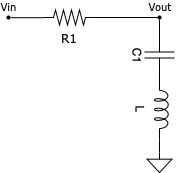
\includegraphics[width=5cm, height=3cm]{../Ex2/Resources/ej2_br.png}
\caption{Rechaza banda}
\label{ej2_filto_BR}
\end{figure}


La función transferencia de este circuito es:

\begin{equation} H(j\omega) = \frac{1-(\frac{j\omega}{\omega_0})^2}{1 - (\frac{\omega}{\omega_0})^{2} + (\frac{j\omega}{\omega_0})\frac{1}{Q}} \label{equ:trans_clasica_br}\end{equation}  

Donde $Q$ es el factor de calidad y $\omega_0$ es la frecuencia de corte.      
Al tener conocimiento de la función transferencia $H(jw)$ es posible proponer un circuito para tratar de obtener una nueva función transferencia que se asemeje lo mas posible a $H(jw)$. 

\subsubsection{Circuito propuesto}
Se propone el circuito de la Figura \ref{fig:ej2_BR_propuesto}. 

%Circuito propuesto
\begin{figure}[!]                                                       
\centering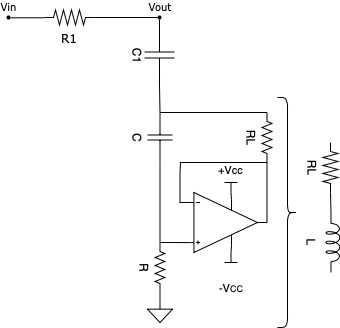
\includegraphics[width=0.4\textwidth, height=4cm]{../Ex2/Resources/ej2_br_gyrator.png}
\caption{Circuito propuesto}
\label{fig:ej2_BR_propuesto}
\end{figure}

Se puede extraer la siguiente función transferencia:

\begin{displaymath} H(s)= \frac{V_{out}}{V_{in}} = \frac{R_L + sL + \frac{1}{sC_1}}{R_L + R_1 +sL + \frac{1}{sC_1}} \end{displaymath}  
\begin{displaymath} H(s)= \frac{sC_1R_L + s^2LC_1 + 1}{s (R_L R_1)C + s^2LC_1 + 1} \end{displaymath}

\begin{displaymath} H(s)= \frac{sC_1R_L + s^2CR_LRC_1 + 1}{s (R_L R_1)C+ s^2CR_LRC_1 + 1} \end{displaymath}




Donde:

\begin{displaymath} \omega_0^2= \frac{1}{CR_LRC_1} \end{displaymath}  
\begin{displaymath} \frac{1}{\omega_0 Q}= (R_L + R_1)C \end{displaymath}  





\subsubsection{Diseño del circuito}


Al igual que en el filtro anterior, se seleccionan los componentes. Como los otros filtros, $R_L = 10 \Omega$ y $ C = 100nF$. En este caso se define $Q = \frac{1}{\sqrt{2}}$,  $C_1 = C$ y $\omega_0 = 2\pi 4k$. 


Gracias a todas estas definiciones se pueden obtener dos ecuaciones que dependen tanto de  $R$ y $R_1$.  

Luego:

\begin{displaymath} R = \frac{1}{C^2 R_L \omega_0^2} = 15831.43 \Omega \end{displaymath}  
\begin{displaymath} R_1 = \frac{1}{\omega_0 Q C} - R_L = 552.69 \Omega \end{displaymath} 


Al tener los valores de todos los componentes, se puede formar la Tabla  \ref{tab:br_gyrator_components} de los componentes utilizados. 

\begin{table}[h!]
\centering
\begin{tabular}{@{}cc@{}}
\toprule
Componente   & Valor \\ \midrule
\text{C}   & 100nF \\
\text{$C_1$}   & 100nF \\
\text{$R_A$}   & $15k\Omega$     \\
\text{$R_B$}   & $820\Omega$     \\
\text{$R_L$} & $10\Omega$    \\ 
\text{$R_1$} & $560\Omega$    \\ \bottomrule
\end{tabular}
\caption{Componentes del circuito propuesto}
\label{tab:br_gyrator_components}
\end{table}



\subsubsection{Simulacion y analisis lineal}
Si se simula el circuito propuesto (desde $f = 1 Hz$ a $f = 10MHz$) con los componentes de la Tabla \ref{tab:br_gyrator_components}, se obtiene el gráfico de la Figura \ref{ej2_br_sim}.

\begin{figure}[h!]                                                       
\centering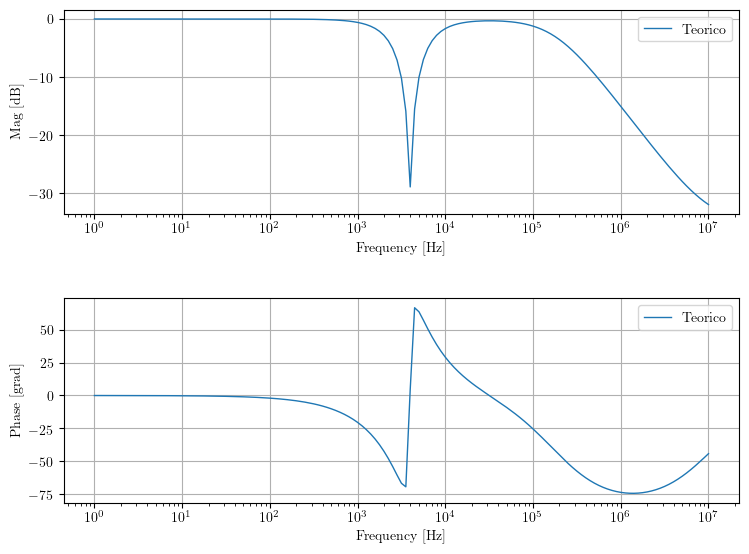
\includegraphics[width=0.9\textwidth, height=9cm]{../Ex2/Resources/ej2_br_sim.png}
\caption{Simulación del circuito propuesto }
\label{ej2_br_sim}
\end{figure}

El bode claramente describe un rechaza banda. La máxima atenuación se da en $f= 4kHz$, que es a la frecuencia deseada. También, cabe destacar que la profundidad del rechaza banda es de aproximadamente $27 dB$. Se puede decir que para ser un filtro pasivo rechaza banda la profundidad obtenida es muy buena.  


Al igual que en la sección anterior, se realiza un análisis lineal. En la Figura \ref{fig:ej2_BR_gyrator_sim} se simula el circuito del \textit{Gyrator} con los correspondientes  $R_A$, $R_B$,  $R_L$ y $C$.



\begin{figure}[h!]                                                       
\centering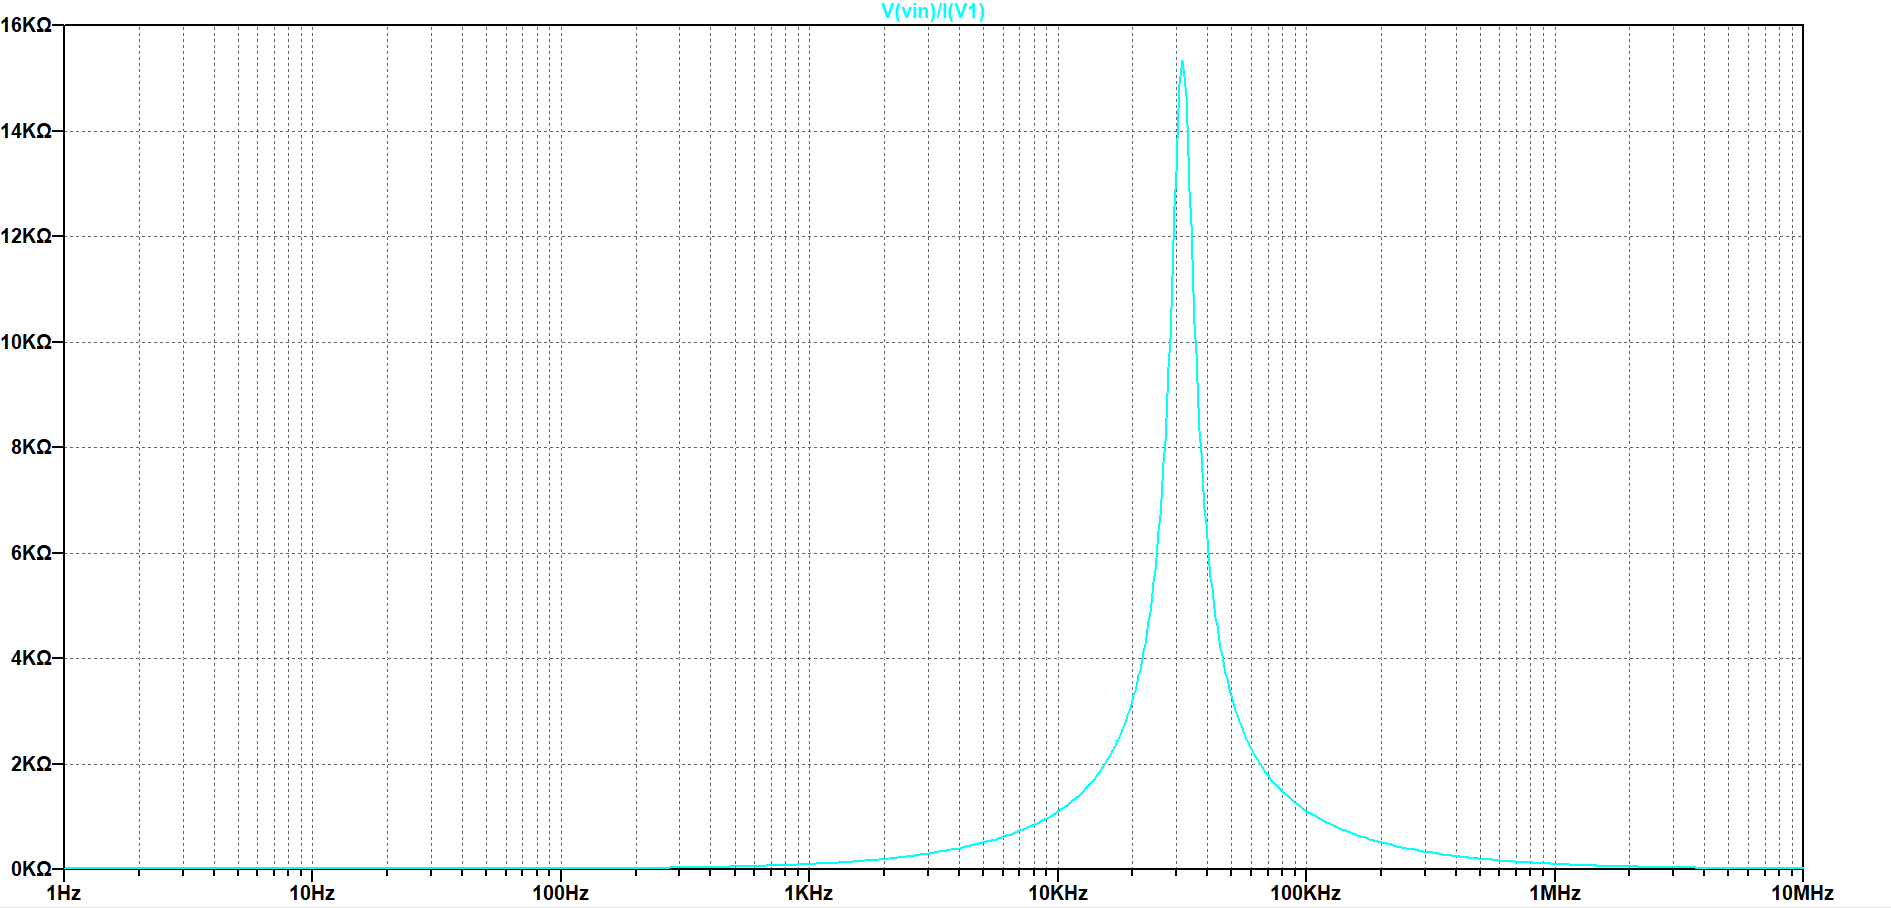
\includegraphics[width=0.9\textwidth, height=7cm]{../Ex2/Resources/ej2_br_gyrator_sim.png}
\caption{Simulación del \textit{Gyrator} }
\label{fig:ej2_BR_gyrator_sim}
\end{figure}


En la simulación del \textit{Gyrator} es muy similar a las simulaciones ya realizadas. En este caso, la impedancia tiene un comportamiento creciente hasta que llega a una frecuencia aproximada de $f = 30 kHz$. Luego, la impedancia cae abruptamente. Como el pico máximo sucede a la frecuencia de $f=4kHz$, se puede decir que el \textit{Gyrator} funciona correctamente en el rango de frecuencias desde bajas frecuencias ($10Hz$) hasta $f = 30kHz$

\subsubsection{Medicion y analisis a altas frecuencias}

Se realiza un bode con una señal de entrada configurada como senoide de $V_{PP} = 3V$ desde $[10Hz , 1MHz]$. La Figura \ref{fig:ej2_hp_med_and_sim}.

\begin{figure}[h!]                                                    
\centering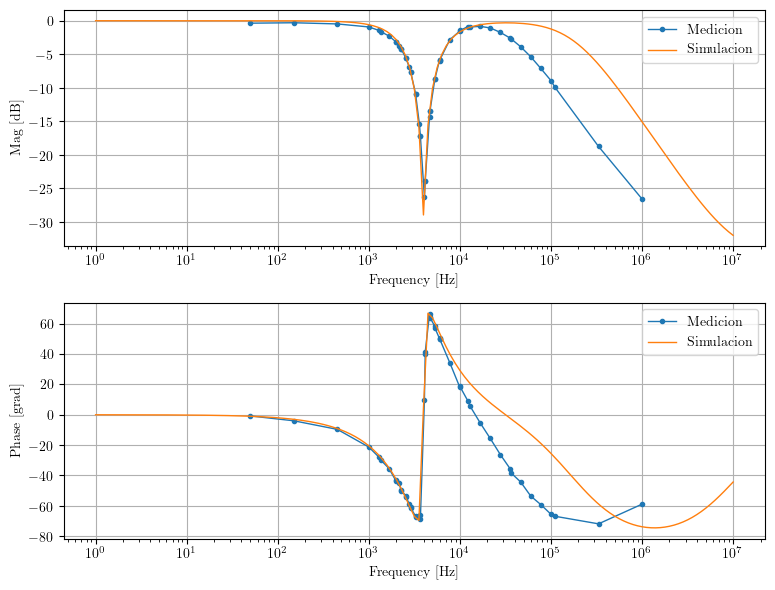
\includegraphics[width=0.9\textwidth, height=9cm]{../Ex2/Resources/ej2_br_med_and_sim.png}
\caption{Bode de medición y simulación}
\label{fig:ej2_hp_med_and_sim}
\end{figure}

Los resultados son satisfactorios. Se destaca que a bajas frecuencias y a la frecuencia del rechaza banda tanto la simulación como la medición se comportan prácticamente igual. Sin embargo, se puede ver que a la frecuencia de $20kHz$, el circuito comienza a atenuar nuevamente. Esto se asemeja con los que se dijo en el análisis lineal. Se predijo que recien $f = 30kHz$ el \textit{Gyrator} deja de funcionar como inductor por lo que, la medición, la atenuación comienza $10kHz$ antes. Este comportamiento se debe por el polo dominante. Recordar que por la condición (\ref{ej2_ecua_condicion_1}) el polo dominante comienza a afectar a $40 kHz$. Lo que sucede se debe a causa de que el \textit{Gyrator} deja de funcionar como bobina y por el polo dominante.  




\subsubsection{Conclusion}

Se cumplió el objetivo de fabricación de un filtro rechaza banda con un \textit{Gyrator}. Ademas, se logro que el filtro se adecue a la plantilla propuesta. Cabe destacar que el filtro cuenta con una profundidad muy buena. El rango de frecuencias de trabajo va desde las bajas frecuencias ($10Hz$) hasta $20kHz$. Lo ideal es que el rechaza banda funcione hasta frecuencias del orden de los $M\Omega$ pero como se vio, por causa del \textit{Gyrator} esto es imposible. 




\subsection{Pasa bajos}

Como ultimo filtro, se intenta fabricar un filtro pasa bajos con un \textit{Gyrator}.


\subsubsection{Plantilla}

\begin{enumerate}
	\item Ganancia unitaria en continua
	\item Ganancia mayor a $-3dB$ para $f<f_p = 4k$
	\item Ganancia menor a $-10dB$ para $f>f_a = 14k$
	\item Ganancia nunca superior a $0dB$
\end{enumerate}

La plantilla se asemeja mucho al filtro pasa altos. En este caso, la frecuencia de corte se situá en $f=4kHz$.

\subsubsection{Funcion transferencia y circuito de segundo orden}

En la Figura \ref{ej2_filto_LP} se puede ver un circuito clásico de un filtro pasa bajos de segundo orden. 

%Grafico clasico RCL
\begin{figure}[h!]                                                       
\centering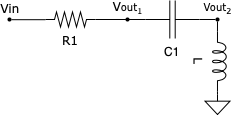
\includegraphics[width=5cm, height=3cm]{../Ex2/Resources/ej2_lp.png}
\caption{Rechaza banda}
\label{ej2_filto_LP}
\end{figure}


La función transferencia de este circuito es:

\begin{equation} H(j\omega) = \frac{1}{1 - (\frac{\omega}{\omega_0})^{2} + (\frac{j\omega}{\omega_0})\frac{1}{Q}} \label{equ:trans_clasica_br}\end{equation}  

Donde $Q$ es el factor de calidad y $\omega_0$ es la frecuencia de corte.      
Al tener conocimiento de la función transferencia $H(jw)$ es posible proponer un circuito para tratar de obtener una nueva función transferencia que se asemeje lo mas posible a $H(jw)$. 

\subsubsection{Circuito propuesto}
Se propone el circuito de la Figura \ref{fig:ej2_LP_propuesto}. 

%Circuito propuesto
\begin{figure}[!]                                                       
\centering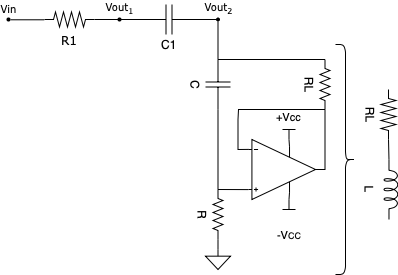
\includegraphics[width=0.4\textwidth, height=4cm]{../Ex2/Resources/ej2_lp_gyrator.png}
\caption{Circuito propuesto}
\label{fig:ej2_LP_propuesto}
\end{figure}


Notar que en la Figura  \ref{fig:ej2_LP_propuesto} hay dos salidas $V_{out}$ que se definen como $V_{out1}$ y $V_{out2}$. Esto se debe a  una de las condiciones del \textit{Gyrator}. Una de las condiciones del circuito propuesto del \textit{Gyrator} es que este conectado a tierra. Entonces, para mantener una consistencia con el resto de los circuitos, se debe obtener la salida de señal del capacitor. Esto se logra simplemente saliendo diferencial del capacitor, realizando $|V_{out1} - V_{out2}|$. 

Teniendo esto en cuenta, se construye la funcion transferencia:

\begin{displaymath} H(s)= \frac{V_{out}}{V_{in}} = \frac{\frac{1}{sC_1}}{R_L + R_1 +sL + \frac{1}{sC_1}} \end{displaymath}  
\begin{displaymath} H(s)= \frac{1}{s (R_L R_1)C + s^2LC_1 + 1} \end{displaymath}

\begin{displaymath} H(s)= \frac{1}{s (R_L R_1)C + s^2  C R_L R C_1 + 1} \end{displaymath}

Donde:

\begin{displaymath} \omega_0^2= \frac{1}{CR_LRC_1} \end{displaymath}  
\begin{displaymath} \frac{1}{\omega_0 Q}= (R_L + R_1)C \end{displaymath}  





\subsubsection{Diseño del circuito}


Al igual que en el filtro anterior, se seleccionan los componentes. Como los otros filtros, $R_L = 10 \Omega$ y $ C = 100nF$. En este caso se define $Q = \frac{1}{\sqrt{2}}$ ya que una de las condiciones del filtro es que nunca se sobrepase $0dB$ También, se define $C_1 = C$ y $\omega_0 = 2\pi 4k$. 


Gracias a todas estas definiciones se pueden obtener dos ecuaciones que dependen tanto de  $R$ y $R_1$.  

Luego:

\begin{displaymath} R = \frac{1}{C^2 R_L \omega_0^2} = 15831.43 \Omega \end{displaymath}  
\begin{displaymath} R_1 = \frac{1}{\omega_0 Q C} - R_L = 552.69 \Omega \end{displaymath} 


Al tener los valores de todos los componentes, se puede formar la Tabla  \ref{tab:lp_gyrator_components} de los componentes utilizados. 

\begin{table}[h!]
\centering
\begin{tabular}{@{}cc@{}}
\toprule
Componente   & Valor \\ \midrule
\text{C}   & 100nF \\
\text{$C_1$}   & 100nF \\
\text{$R$}   & $15k\Omega$     \\

\text{$R_L$} & $10\Omega$    \\ 
\text{$R_1$} & $510\Omega$    \\ \bottomrule
\end{tabular}
\caption{Componentes del circuito propuesto}
\label{tab:lp_gyrator_components}
\end{table}


\subsubsection{Simulacion y analisis lineal}
Si se simula el circuito propuesto (desde $f = 1 Hz$ a $f = 10MHz$) con los componentes de la Tabla \ref{tab:lp_gyrator_components}, se obtiene el gráfico de la Figura \ref{ej2_lp_sim}.

\begin{figure}[h!]                                                       
\centering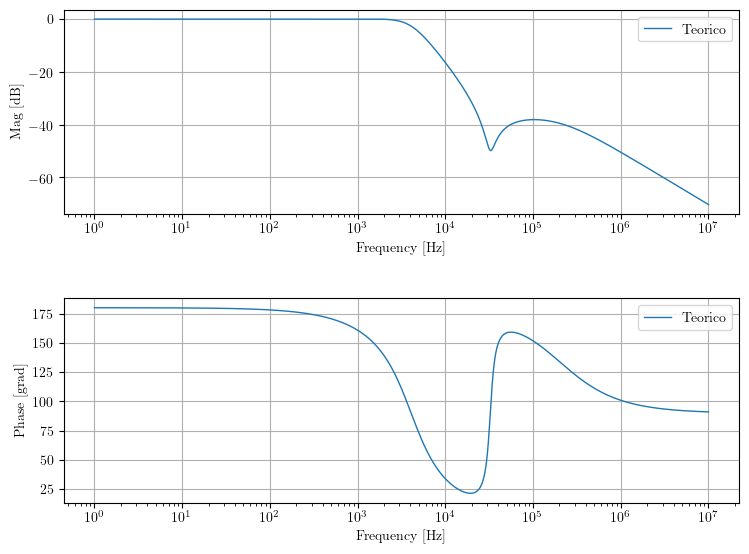
\includegraphics[width=0.9\textwidth, height=9cm]{../Ex2/Resources/ej2_lp_sim.png}
\caption{Simulación del circuito propuesto }
\label{ej2_lp_sim}
\end{figure}

El bode describe un comportamiento de pasa bajos. 


A la frecuencia de corte de $f= 4kHz$, la atenuación es de $2.55 dB$. Si bien no es $3dB$, la configuración cumple con la condicion 2.  También, se logra cumplir con la condición 1, 3 y 4. Se prosigue al análisis lineal. En la Figura \ref{fig:ej2_LP_gyrator_sim} se simula el circuito del \textit{Gyrator} con los correspondientes  $R_A$, $R_B$,  $R_L$ y $C$.



\begin{figure}[h!]                                                       
\centering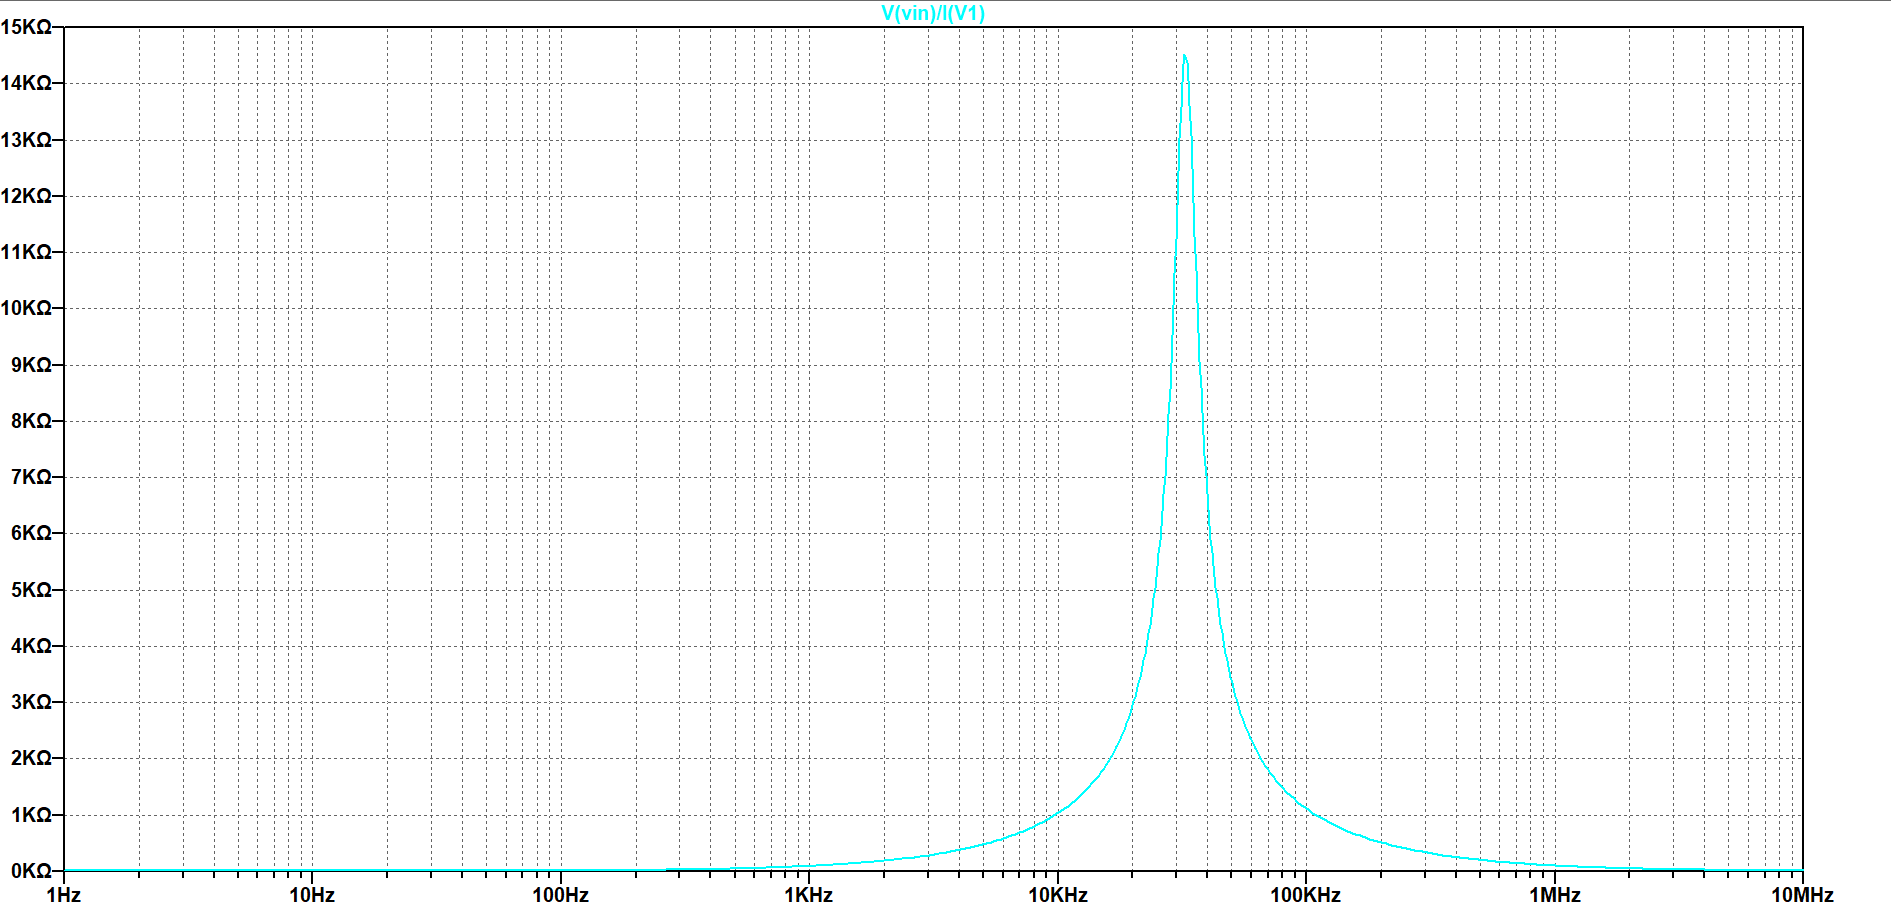
\includegraphics[width=0.9\textwidth, height=7cm]{../Ex2/Resources/ej2_lp_gyrator_sim.png}
\caption{Simulación del \textit{Gyrator} }
\label{fig:ej2_LP_gyrator_sim}
\end{figure}

Nuevamente el \textit{Gyrator} describe un comportamiento de impedancias muy similar a las simulaciones ya realizadas. El pico máximo se da en $14 kHz$. Como se desea que el \textit{Gyrator} funcione apropiadamente en la frecuencia de corte ($4kHz$), se puede decir que el 
\textit{Gyrator} funciona correctamente para el rango de frecuencias deseadas y al sobrepasar $f = 4 kHz$ dejara de actuar como una bobina. Por esta razon a la frecuencia de $f=30kHz$ se observa una disminucion en la atenuacion. La misma dura en un rango acotado y ademas no provoca que las condiciones de la plantilla no se cumplan por lo que no se analisa con mayor profundidad. 


\subsubsection{Medicion y analisis a altas frecuencias}

Al imponer una senoide de $V_{PP} = 3V$ como señal de entrada al circuito en un rango de frecuencias de $[10Hz , 1MHz]$, se obtiene el bode de la Figura \ref{fig:ej2_lp_medicion}.

\begin{figure}[h!]                                                       
\centering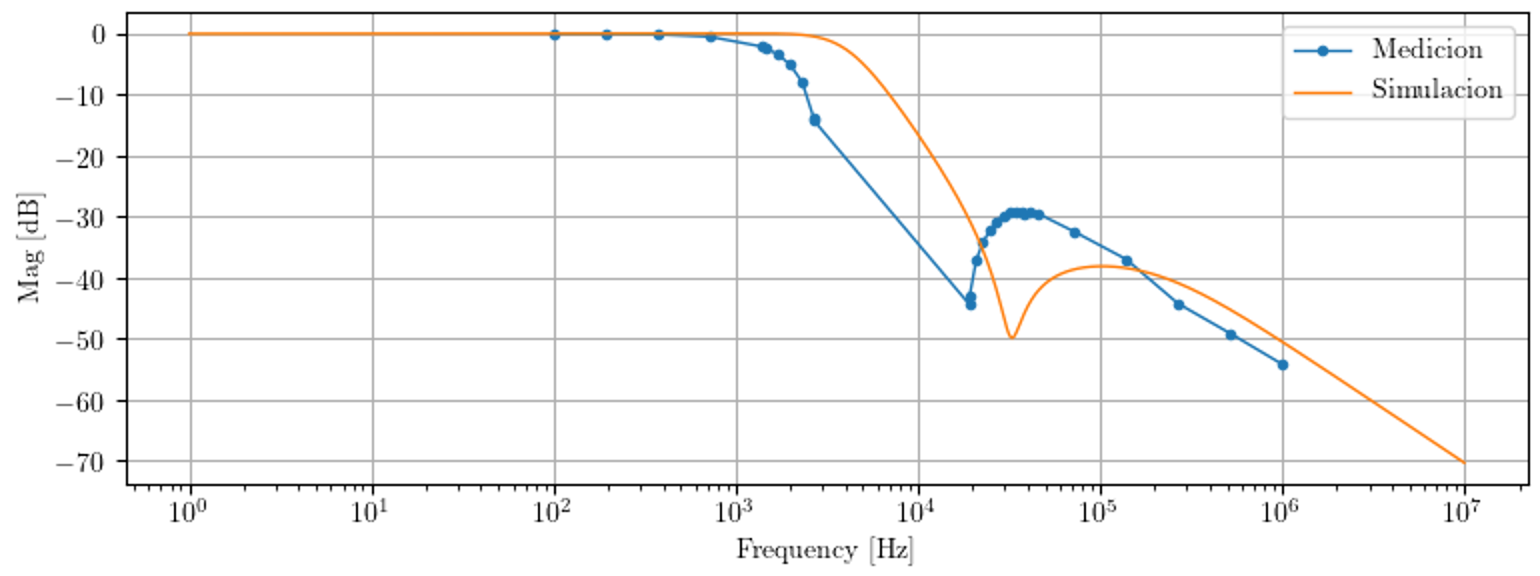
\includegraphics[width=0.9\textwidth, height=7cm]{../Ex2/Resources/ej2_lp_med_and_sim.png}
\caption{Medición y simulación del circuito propuesto }
\label{fig:ej2_lp_medicion}
\end{figure}

Como se puede ver, se superponen en el gráfico tanto la simulación como la medición. A diferencia del resto se aprecia un corrimiento de la medicion con respecto a la simulacion. Sin embargo, como la medicion tambien cumple con la plantilla del filtro esto no es un inconveniente. Al igual que el pasa banda, la condicion (\ref{ej2_ecua_condicion_2}) no es de importancia ya que el polo dominante atenua a altas frecuencias y como se trata de un pasa bajos esto es una condicion favorable. 

\subsubsection{Conclusion}

Si bien para obtener un pasa bajos se tuvo que salir de modo diferencial del capacitor, se logro cumplir la plantilla propuesta. Gracias a la implementación del \textit{Gyrator} se logro obtener un filtro pasa bajos. El filtro cumple con las condiciones de la plantilla para todo el rango de frecuencias evaluado $[10Hz,10MHz]$.


\section{Diseño PCB}

Para realizar todos los filtros mencionados a lo largo de las secciones se decide diseñar un PCB que contenga los cuatro filtros y que utilice el mismo integrado (TL084). En la Figura \ref{fig:pcb} se ve dicho diseño. 

\begin{figure}[h!]                                                       
    \centering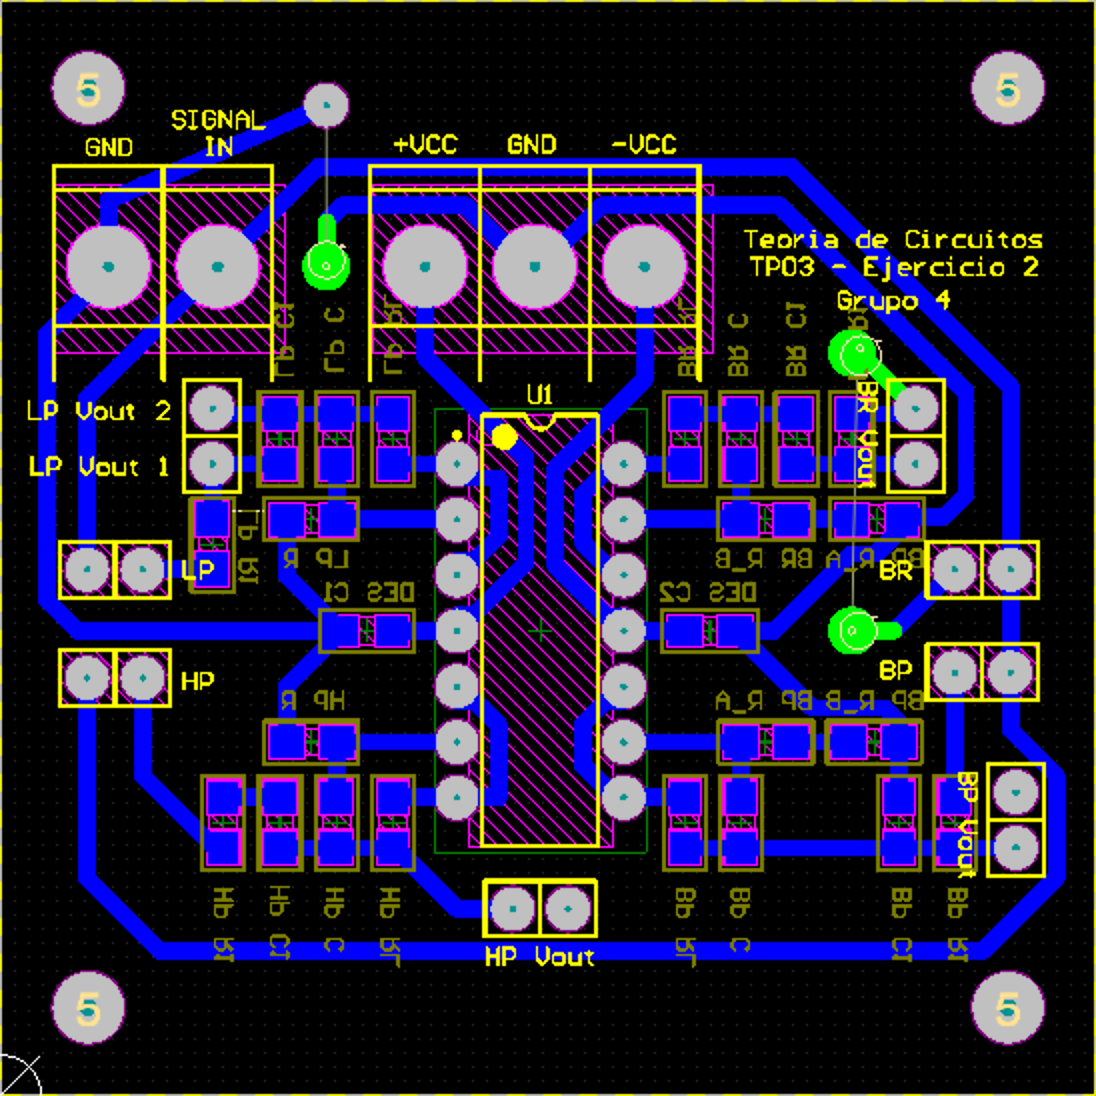
\includegraphics[width=7cm, height=7cm]{../Ex2/Resources/ej2_pcb.png}
    \caption{Diseño del PCB }
    \label{fig:pcb}
    \end{figure}
    



